\documentclass[12pt]{article}
\usepackage[margin=1.25in]{geometry}
\usepackage{mathrsfs}
\usepackage[title,toc,titletoc]{appendix}
\usepackage{titlesec}
\titleformat{\section}[block]{\large\normalfont\filcenter}{\thesection.}{.5em}{}
\titleformat{\subsection}[hang]{\itshape\bfseries}{\thesubsection.}{.5em}{}
%\titlespacing*{\section}
%{0pt}{1\baselineskip}{1\baselineskip}
%\titlespacing*{\subsection}
%{0pt}{1\baselineskip}{1\baselineskip}
\usepackage[dvipsnames]{xcolor}
\usepackage{bbm}
\usepackage{bm}
\usepackage{amsmath, amssymb}	
% \usepackage{dutchcal}
\usepackage[shortlabels]{enumitem}
\usepackage[hang,flushmargin]{footmisc}
\usepackage[round]{natbib}
\usepackage[colorlinks=true,linkcolor = blue, citecolor=blue, hyperfootnotes=false, hyperindex,breaklinks]{hyperref}
\usepackage{cleveref}
\usepackage{bigints}
\newcommand{\definitionautorefname}{Definition}
\newcommand{\lemmaautorefname}{Lemma}
\newcommand{\remarkautorefname}{Remark}
\newcommand{\corollaryautorefname}{Corollary}
\newcommand{\propositionautorefname}{Proposition}
\newcommand{\exampleautorefname}{Example}
\usepackage{pgf}
\usepackage[justification=centering]{caption}
\usepackage{subcaption}
\usepackage{tikz}
\usetikzlibrary{patterns, decorations.pathreplacing}
\usepackage{hhline}
\usepackage{float}
\usepackage{siunitx}
\usepackage{textcomp}
\usepackage[subtle]{savetrees}
\usepackage{graphics}
\usepackage{graphicx}
\def\tm{\textcolor{red}}
\def\bph{\textcolor{cyan}}
\def\zma{\textcolor{orange}}

\newtheorem{theorem}{Theorem}
\newtheorem{proposition}{Proposition}
\newtheorem{claim}[proposition]{Claim}
\newtheorem{axiom}{Axiom}
\newtheorem{remark}{Remark}
\newtheorem{corollary}{Corollary}
\newtheorem{definition}{Definition}
\newtheorem{lemma}{Lemma}
\newtheorem{assumption}{Assumption}
\newenvironment{proof}[1][Proof]{\textbf{#1.} }{\  \rule{0.5em}{0.5em}}
\DeclareMathOperator*{\argmax}{arg\,max}
\DeclareMathOperator*{\argmin}{arg\,min}
\DeclareMathOperator*{\inte}{int}
\DeclareMathOperator*{\supp}{supp}
\renewcommand{\arraystretch}{1.5}
\usepackage{setspace}
\usepackage{multirow}
\definecolor{shade}{gray}{.7}
\onehalfspacing
\frenchspacing

\newcommand\blfootnote[1]{%
  \begingroup
  \renewcommand\thefootnote{}\footnote{#1}%
  \addtocounter{footnote}{-1}%
  \endgroup
}

\begin{document}
\title{Persuaded Search\thanks{For helpful comments and discussions, we thank Nageeb Ali, Nima Haghpanah, Emir Kamenica, Erik Madsen, Andy Skrzypacz, Juuso Toikka, Mark Whitmeyer, Kun Zhang, and seminar audiences at Brown,  Duke, NYU Stern, Princeton, Conference on Mechanism and Institution Design, Cowles Conference on Economic Theory, SITE, and Stony Brook International Conference on Game Theory. This paper supersedes a previous draft entitled ``Certification in Search Markets.''}}
\author{Teddy Mekonnen\thanks{Department of Economics, Brown University. Contact: \href{mailto:mekonnen@brown.edu}{mekonnen@brown.edu}}\hspace*{1.25em} Zeky Murra-Anton\thanks{Market Development, ISO New England. Contact: \href{mailto:zmurraanton@iso-ne.com }{zmurraanton@iso-ne.com}. This paper has not been funded or endorsed by ISO New England nor does it represent ISO New England's views.} \hspace*{1.25em} Bobak Pakzad-Hurson\thanks{Department of Economics, Brown University. Contact: \href{mailto:bph@brown.edu}{bph@brown.edu}}}
\date{\today}


\maketitle
\thispagestyle{empty}
\setcounter{page}{0}
\begin{abstract}
We consider sequential search by an agent who cannot observe the quality of goods but can acquire information by buying signals from a profit-maximizing principal with limited commitment power. The principal can charge higher prices for more informative signals in any period, but high prices in the future discourage continued search by the agent, thereby reducing the principal's future profits. A unique stationary equilibrium outcome exists, and we show that the principal $(i)$ induces the socially efficient stopping rule, $(ii)$ extracts the full surplus, and $(iii)$ persuades the agent against settling for marginal goods, extending the duration of surplus extraction. However, introducing an additional, free source of information can lead to inefficiency in equilibrium.
\end{abstract}


\noindent \textit{JEL Classifications: D83, D86, L15}\\
\noindent\textit{Keywords: search, information design, information acquisition}
\newpage

\section{Introduction}\label{intro}
 \begingroup
\allowdisplaybreaks
Agents in search and matching markets often contend with frictions stemming from incomplete information. An agent who does not perfectly observe the quality of the goods he samples during his search may mistakenly select a good of inferior quality or may abandon his search altogether. Given these inefficiencies, it is unsurprising that searching agents turn to information brokers so as to reduce the inherent uncertainty in various markets: consumers seek information on products before making purchases, home buyers commission geological risk assessments for natural disasters before closing, and individuals turn to advice from matchmakers to identify compatible spouses.\footnote{Each author of this paper has solicited CarFax reports during searches for used automobiles. Two authors have commissioned geological reports while searching for houses. None of the authors admits to having contacted a matchmaker, but at least one probably should.} 


To fix ideas, consider a firm seeking to fill a job vacancy. The firm may not perfectly observe a candidate employee's  productivity. Yet, the firm can contract with an information broker who adjudicates the candidate's productivity through skill assessments and job simulations. 82\% of US private-sector firms use such pre-employment testing services,\footnote{https://www.sparcstart.com/wp-content/uploads/2018/03/2017-CandE-Report.pdf.}  giving rise to an industry with 2 billion USD in annual revenue.\footnote{https://www.polarismarketresearch.com/industry-analysis/candidate-skills-assessment-market. The annual revenue figure is given for the most recent year reported, 2021, and  is projected to nearly triple by 2030.} Evidence shows that pre-employment testing  dramatically increases the quality of worker hired, and provides significant information to the firm that is otherwise unavailable at the time of hiring \citep{aut08, hof18}. In some cases, like low-skill service jobs, the candidate assessment plays a crucial role in the hiring process, as it typically occurs before the job interview,\footnote{https://www.sparcstart.com/wp-content/uploads/2018/03/2017-CandE-Report.pdf.} and the test results often serve as the deciding factor in hiring decisions.\footnote{\cite{hof18} show that firms which base their hiring decisions solely on pre-employment test results outperform firms that base their decisions either on pre-employment tests along with interviews or only on interviews. \cite{aut08} suggest that pre-employment test results affect only hiring and not wages in the particular market they study. More broadly, test results are typically not revealed to candidate employees and are therefore unlikely to factor into wage setting.} Firms often contract with information brokers on a short-term basis, possibly due to difficulties committing to future assessments in the presence of changing skill demands over time.\footnote{For example, ProfileXT charges per worker assessed. Criteria sells a monthly subscription to its assessment service.}

We refer to the interaction between a searching ``agent" (he) and a ``principal" (she) who brokers information as a \emph{persuaded search} game. The principal only makes money as long as the search continues, and only if the information sold is useful in the search process. However, the information provided, and the price charged, can potentially affect the duration of search. The difference in the objectives of the two parties leads to natural questions:  How much information should the principal optimally convey? How much should she charge? How do the answers to these questions change depending on the amount of exogenous information available about each good in the search market?

% We study these questions in a parsimonious model that embeds a standard information design framework \`a la \cite{kam11} into a simple sequential search problem \`a la \cite{mcc70}. In our model, a long-lived {agent} (he)  seeks to fill a single vacancy by randomly sampling from a continuum of goods that are differentiated in their quality. The agent considers one good per period and exits the market upon making a selection. The agent prefers to match with a higher quality good but is also impatient and prefers to match sooner rather than later.\footnote{Our main result goes through with only subtle differences if impatience is modeled via exponential discounting or via a flow cost for searching. These are the primary ways impatience is modeled in the search literature.} We depart from the classic sequential search literature by assuming that the agent cannot directly observe the quality of a sampled good. Instead, he may acquire information by purchasing a signal from a long-lived, profit-maximizing  {principal} (she). The principal  picks the informativeness of the signal and sells it by offering a spot contract to the agent, and we assume that she has limited commitment power in the sense that she is unable to commit to contracts beyond the current period.   

To answer these questions, we propose a parsimonious model that embeds an information design framework \`a la \cite{kam11} into a simple sequential search problem \`a la \cite{mcc70}. In our model, a long-lived agent  seeks to fill a single vacancy by randomly sampling from a continuum of goods that are differentiated in their quality. The agent considers one good per period and exits the market upon making a selection. The agent prefers to match with a higher quality good but is also impatient and prefers to match sooner rather than later.\footnote{Our main result goes through with only subtle differences if impatience is modeled via exponential discounting or via a flow cost for searching. These are the primary ways impatience is modeled in the search literature.} We depart from the classic sequential search literature by assuming that the agent cannot directly observe the quality of a sampled good. Instead, he can acquire information from a long-lived  principal. We also depart from much of the information design literature by assuming that the principal has no intrinsic  preferences over the outcome of the agent's search. Instead, the principal sells information to the agent and seeks to maximize her profits. In each period, she picks the informativeness of a signal and sells it by offering a spot contract to the agent, and we assume that she has limited commitment power in the sense that she is unable to commit to contracts beyond the current period.   



In any given period, the principal's payoff is derived from the profit she earns in that period, which depends on the spot contract she offers, and her value from a continued relationship with the agent, which depends on the contracts she will offer in the subsequent periods. The dynamic nature of the agent’s search problem gives rise to two important considerations for the principal's profit maximization. First, for a fixed sequence of future contracts, she must contend with an \emph{intra-temporal} trade-off between surplus extraction and persuasion: the principal can earn a higher profit today by selling a Blackwell more informative signal, but a more informative signal can lower the probability with which the agent is persuaded  to continue his search. Second, contracts offered in subsequent periods have \emph{inter-temporal} impacts on the trade-off between extraction and persuasion in the current period: higher prices or less informative signals in the future lower the agent's value from continued search, thereby reducing both his willingness-to-pay (WTP) for information today (and thus the surplus that can be extracted today), and his willingness to continue searching today (and thus the principal's ability to persuade him). We study stationary equilibria in which the same spot contract must resolve the intra-temporal trade-off in each period while also taking into account its inter-temporal impact.

Our main result shows that in any stationary equilibrium, the principal fully extracts the socially efficient surplus, i.e. 
 the maximum expected surplus that can be generated from search. Efficiency implies that the agent searches as if he receives full information for free; he terminates his search if and only if a good's quality exceeds the \emph{McCall reservation value}--the same reservation value used by the agent in \cite{mcc70}. In contrast, surplus extraction implies that the agent is no better off than in autarky, that is, searching without any information. As the agent earns his autarky payoff, he would prefer to terminate his search for any good whose expected quality exceeds the \emph{autarky reservation value}--the reservation value the agent would use without any signal of a good's quality. The McCall reservation value exceeds the autarky reservation value, implying that the agent searches longer than he would otherwise prefer in equilibrium.


Surplus extraction is intuitive in our setting; the agent lacks any bargaining power because the principal designs the contract in each period. Furthermore, in a stationary equilibrium, the agent cannot use the threat of low continuation payoffs to prevent profitable deviations by the principal. 

What is more surprising is that a principal with limited commitment can nevertheless generate the socially efficient surplus and simultaneously extract it. In order to achieve this outcome in a stationary equilibrium, the principal offers a spot contract with two prominent and interdependent features. First, the principal  persuades the agent against an early exit from the search market by pooling goods with qualities below the McCall reservation value into a ``fail" signal realization.\footnote{Such pooling signals are in line with the pre-employment testing studied in \cite{aut08}. They document that while the assessments generate a rich set of test scores, the information broker pools low performers into an implicit ``fail" category (the probability of being hired conditional on inclusion in this category is 0.08\%).}  The implementability of this pooling signal crucially hinges on the agent's incentives to continue his search when he sees ``fail" and to stop his search otherwise. It is intuitive to see that the agent is persuaded to stop his search when he does not observe a ``fail." We show that by pooling goods whose qualities fall between the autarky and McCall reservation values (sufficiently high quality goods for which the agent would be willing to stop his search) with goods whose qualities fall below the autarky reservation value (low quality goods for which he would rather continue searching), the agent is persuaded to continue searching when he observes a ``fail."

Second, the per-period price the principal charges for this pooling signal is equal to the agent's WTP for it, implying that the agent's participation constraint binds. In general, this per-period price is a fraction of the expected total profit the principal derives. Consequently, the principal extracts the entire surplus through dribs and drabs over a long period of time.

Our model of persuaded search thus far, in which the principal is the sole source of information, yields a stark prediction; the principal neither gains from considering more complex history-dependent contracts nor has any value for commitment as she extracts the maximum possible surplus by offering the same  contract in each period both on and off the equilibrium path.

To capture a feature present in many real-world search markets as well as to understand the limiting factors to full surplus extraction, we extend our model of persuaded search to the case when some information is available even without contracting with the principal. For example, a job candidate with a  college degree is informationally differentiated from a job candidate without a college degree. Formally, we study a setting in which an exogenous signal of each good's quality is publicly observed immediately upon sampling and prior to contracting with the principal, inducing potentially heterogeneous interim beliefs. The principal then offers a spot contract that can depend on the realization of the public signal (e.g., providing a different skill-assessment to those with versus without college degrees).


While the agent is ex-ante (weakly) better off in equilibrium when he has accesss to a free and public signal, we show that he may nonetheless end up with an ex-post lower-quality match, giving rise to inefficiencies.  To understand the equilibrium effects of a public signal, recall that the principal desires to both charge the agent a high price and to keep the agent in the market as long as possible.  As the public signal mechanically increases the agent's autarky payoff, its presence erodes the principal's profits. Moreover, the realized public signal could induce interim beliefs that are either 
\textit{pessimistic}\textemdash revealing the sampled good is of sufficiently low quality that the agent rejects it regardless of any additional information\textemdash or \textit{optimistic}\textemdash revealing the sampled good is of sufficiently high quality that the agent stops his search and consumes it regardless of any additional information. In either case, the agent has zero WTP for any signal the principal offers.

% Even if the agent has a positive WTP for additional information following some realization of the public signal, the presence of the  public signal could still have welfare consequences by affecting the duration of search. Once again, consider the pooling signal that ``fails" goods below the McCall reservation value. If the agent's interim posterior belief has a sufficiently \textit{fat right tail}\textemdash a high probability mass on the sampled good's quality being high\textemdash then even conditional on observing a ``fail," the expected quality of the good is high enough that the agent strictly prefers to stop his search and consume the good. In order to persuade the agent to continue searching, the principal cannot ``fail" all goods with qualities below the McCall reservation value, thus distorting the agent's search behavior away from the efficient outcome. When the agent's interim belief has a fat right tail, the optimal spot contract completely gives up on surplus extraction and fully prioritizes persuasion; the principal ``fails" as many goods with qualities below the McCall reservation value as possible while still persuading the agent, and gives this signal away for free.

Even if the agent has a positive WTP for additional information following some realization of the public signal, the presence of the  public signal could still have welfare consequences by affecting the duration of search. Once again, consider the pooling signal that ``fails" goods below the McCall reservation value. If the agent's interim posterior belief has a sufficiently \emph{thin left tail}\textemdash  lower mass below the autarky reservation value than between the autarky and the McCall reservation values\textemdash then even conditional on observing a ``fail," the expected quality of the good is high enough that the agent strictly prefers to stop his search and consume the good. In order to persuade the agent to continue searching, the principal cannot ``fail" all goods with qualities below the McCall reservation value, thus distorting the agent's search behavior away from the efficient outcome. In this case, the optimal spot contract completely gives up on surplus extraction and fully prioritizes persuasion; the principal ``fails" as many goods with qualities below the McCall reservation value as possible while still persuading the agent, and gives this signal away for free.

We show that a public signal gives rise to inefficiency if and only if it induces interim beliefs that are either  optimistic or have thin left tails. We also provide a necessary and sufficient condition under which the principal extracts the full surplus in a stationary equilibrium in the presence of a public signal.




\subsection*{Related Literature}
Our paper marries the literature on sequential search with the more recent literature on information design. There is a small but growing body of work at the intersection of these two literatures. In the context of random search markets, \cite{do22} and \cite{hu22} consider a centralized information design problem in which a planner shapes the price competition between firms by controlling the information about the quality of goods that the consumers observe, while \cite{boa19} and \cite{whi21} consider a decentralized information design problem wherein each firm competes by choosing how much information it discloses to consumers. \cite{au2023attraction} similarly study firm competition in prices and information but in the context of directed search markets.\footnote{\cite{an06} and \cite{ch19} study information design for a search good, whose true value is revealed upon sampling. In these models, the information designer seeks to persuade an agent to engage in search. Our model crucially differs in that we study search for an experience good whose true value is revealed only upon consumption following the termination of search. Therefore, our principal seeks to persuade the agent to continue his search.}


Our work differs from these papers in two ways: First, in all the aforementioned  papers, information itself is not for sale; it is merely a tool for impacting the price and the selling probability of a separate good. In contrast, the main focus of our paper is precisely the design and pricing of information as a good. Second, 
 the relationships in all these papers are short term: if a consumer and a firm fail to trade, both move on to new trading partners. In contrast, a key feature of our framework is that the relationship between the agent and the principal is long term, which allows us to study the inter-temporal effects of repeated contracting. These dynamic effects also differentiate our paper from the related literature on the design and pricing of information goods \citep{adm86, adm90, es07,ber15, ber18}  and the literature on certification \citep{mat85,sha94,liz99, ali22}, which all focus on static problems. 
 
 Information design with long-term relationships have also been studied by \cite{hor16}, \cite{orl20}, and \cite{ely20}. A common feature is that there is a persistent state that is unobserved by the agent, which leads to a non-stationary contractual environment because the agent becomes more informed over time. In all three, commitment power plays an important role in equilibrium outcomes. Our model does not feature cumulative learning by either the agent or the principal as the underlying environment is stationary, and we show that the principal cannot improve on her stationary equilibrium payoffs with commitment power.
 % \footnote{In a different setting, \cite{ben2019mechanisms} show that commitment is unnecessary in mechanism design problems with evidence disclosure.} 



The information design literature has focused on two prominent representations of information: one is a representation of information as distributions of posterior beliefs or posterior means subject to a Bayes-plausibility constraint \citep{kam11, gen16, kol18, dwo19, iva21} and the other is a representation of information as mechanisms with action recommendations subject to obedience constraints \citep{bergemann2016bayes, bergemann2019information, perez2022test}. We take the former approach because it allows us to resolve an optimization and a fixed point problem simultaneously, providing a tractable way to characterize all equilibrium signals (including some that are strictly Blackwell more informative than recommendations). From an expostitional point, this method also enables a geometric intuition of the trade-offs tackled in our paper.

The rest of the paper is organized as follows: We describe our model in \hyperref[model]{\Cref{model}} and introduce analytical tools in \hyperref[prelim]{\Cref{prelim}}. We then present our main result in \hyperref[stationary]{\Cref{stationary}} and extend our analysis to include public signals in \hyperref[public]{\Cref{public}} before concluding in \hyperref[conclude]{\Cref{conclude}}. Omitted proofs are located in the \hyperref[appendix]{Appendix}, and we include extensions of our model to allow for flow search costs and unequal discount factors in the Online Appendix.

\section{Model}\label{model}
We consider an information design problem that is embedded in a sequential search problem without recall. The game involves a market comprised of a continuum of goods differentiated by quality, an agent (he) who searches within the market for a good to consume, and a principal (she) who controls the information the agent observes while he searches.  

The quality of a good, which we denote by $\theta$, is  identically and independently distributed according to an absolutely continuous distribution $F$ on an interval $[\underline\theta, \bar\theta]\triangleq \Theta$ with $\infty>\bar\theta>\underline \theta>-\infty$. We denote the prior expected quality by  $\mathbb{E}_F[\theta]\triangleq m_\varnothing$ and assume that $m_\varnothing>0$.\footnote{Our results do not depend on the sign of $m_\varnothing$. We make this assumption to simplify the exposition.  }

    The agent has unit demand and his ex-post payoff from consuming a good equals the good's quality. In each period $t=1, 2,\ldots$ that the agent remains in the market, he samples a good of quality $\theta_t$ uniformly at random from the continuum of goods, with neither the agent nor the principal observing the good's true quality. The principal then offers a contract $\langle p_t, (\pi_t, S_t)\rangle$ consisting of a price $p_t\in\mathbb{R}_+$ and a signal $(\pi_t, S_t)$ where $\pi_t:\Theta\to \Delta(S_t)$ is a mapping from a good's true quality to a probability distribution over a compact set of possible signal realizations $S_t$. The principal can design any signal in any given period but she has limited commitment, i.e.,  she cannot commit to contracts beyond the current period. The agent either accepts or rejects the contract. If the agent accepts the contract $(a_t=1)$, he pays $p_t$ and observes a signal realization $s_t\in S_t$ distributed according to $\pi_t(\theta_t)$. If the agent instead rejects the contract $(a_t=0)$, he pays nothing and observes no signal. Finally, the agent decides whether to consume the sampled good and stop searching $(d_t=1)$, in which case the game ends, or to continue searching $(d_t=0)$, in which case the game continues on to $t+1$.\footnote{Our model does not allow the agent to  recall a previously sampled good. Consider a richer model in which the agent can recall goods and the principal observes whenever a good is recalled. For any stationary equilibrium of the base game we study, there exists an equilibrium of this richer model in which 1) the principal provides no new information for any recalled good, 2) the agent never recalls on path, and 3) both players receive the same payoffs. } The agent and the principal have a common discount factor $\delta\in (0,1)$.   \autoref{fig:timing} depicts the timing of events within a period and \autoref{tab:payoffs} presents the per-period payoffs.

\begin{figure}[ht]
\centering 
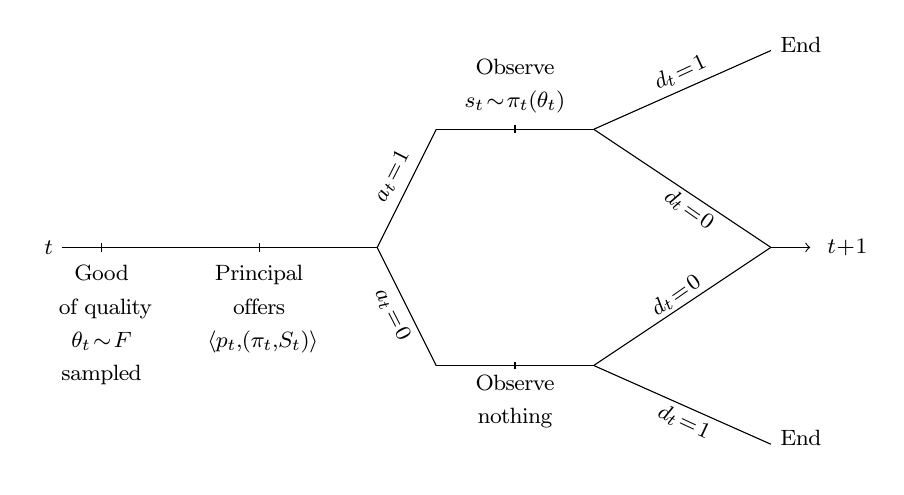
\begin{tikzpicture}[scale=0.5]
\tikzset{
    position label/.style={
             text depth = 1ex
    }
}
    \foreach \x in {-5, -1}
      \draw (\x cm,3pt) -- (\x cm,-3pt);
\draw[-] (-6,0) node[left]{\footnotesize{ $t$}}--(2,0);
\draw[-] (2,0)--(3.5,3);
\draw[-] (2,0)--(3.5,-3);
\draw[-] (3.5,-3)--(7.5,-3);
\draw[-] (3.5,3)--(7.5,3);
\draw[-] (7.5,-3)--(12,0);
\draw[-] (7.5,-3)--(12,-5);
\draw[-] (7.5,3)--(12,5);
\draw[-] (7.5,3)--(12,0);
\draw[->] (12,0)--(13,0)node[right]{\footnotesize{ ${t+1}$}};

\node [position label, align=center, below=3pt] (fend) at (-5,0) {\footnotesize{Good} \\ \footnotesize{ of quality}\\ \footnotesize{$\theta_t\sim F$}\\ \footnotesize{sampled}};
\node [position label, align=center, below=3pt] (fend) at (-1,0) {\footnotesize{Principal} \\ \footnotesize{offers}\\ \footnotesize{ $\langle p_t, (\pi_t, S_t)\rangle$}};
\node [position label, rotate=63, align=center, above] (fend) at (3,1.5) {\footnotesize{$a_t=1$}};
\node [position label, rotate=297, align=center, below] (fend) at (2.8,-1.5) {\footnotesize{$a_t=0$}};


\draw[](5.5,3.1)--(5.5,2.9);
\draw[](5.5,-3.1)--(5.5,-2.9);


\node [position label, align=center, above] (fend) at (5.5,3) {\footnotesize{Observe}\\ \footnotesize{$s_t\sim\pi_t(\theta_t)$}};
\node [position label, align=center, below] (fend) at (5.5,-3) {\footnotesize{Observe}\\ \footnotesize{nothing}};

% \draw[](13,3.1)--(13,2.9);
% \draw[](13,-3.1)--(13,-2.9);
\node [position label, align=center, right] (fend) at (12,5) {\footnotesize{End}};
\node [position label, align=center, right] (fend) at (12,-5) {\footnotesize{End}};

\node [position label, rotate=335, align=center, below] (fend) at (10,-4) {\footnotesize{$d_t=1$}};
\node [position label, rotate=35, align=center, above] (fend) at (10,-1.8) {\footnotesize{$d_t=0$}};

\node [position label, rotate=25, align=center, above] (fend) at (10,3.8) {\footnotesize{$d_t=1$}};
\node [position label, rotate=325, align=center, below] (fend) at (10.2,1.35) {\footnotesize{$d_t=0$}};
  \end{tikzpicture}
  \caption{Timing of events}
  \label{fig:timing}
\end{figure} 

\begin{table}[ht]
\begin{center}
    \begin{tabular}{c|c|c}
         & $a_t=1$& $a_t=0$ \\[8pt] \hline \hline
        $d_t=1$ & $\theta_t-p_t, p_t$& $\theta_t, 0$\\[8pt] \hline
        $d_t=0$& $-p_t, p_t$ & $0,0$
    \end{tabular}
    \caption{Period-$t$ payoffs for the agent and the principal, respectively.}
    \label{tab:payoffs}
    \end{center}
\end{table}

We investigate stationary (Perfect Bayesian) equilibrium outcomes of this game, which are  characterized by a strategy specifying contract proposal for the principal, a strategy specifying contract acceptance and search stopping for the agent, and a belief-updating process such that $(i)$  strategies are stationary, i.e.,  history-independent both on and off the equilibrium path, $(ii)$ strategies are sequentially rational, and $(iii)$ beliefs are derived by Bayes rule. We provide a more formal definition after we define the contract space. 

\section{Preliminary Analysis}\label{prelim}
\subsection{Signals as posterior-mean distributions}
Suppose the principal proposes a period-$t$ contract $\langle p_t, (\pi_t, S_t)\rangle$ and the agent rejects. The agent's period-$t$ payoff would then be zero if he continues to search whereas his expected payoff would be $m_\varnothing$ if he consumes the good and ends the game. In contrast, if the agent accepts the contract and observes a signal realization $s_t\in S_t$, he would update his belief about the good's quality from his prior $F$ to a posterior  $F_{s_t}^{\pi_t}$  using Bayes rule. The posterior mean would then be $\mathbb{E}_{F^{\pi_t}_{s_t}}[\theta]$, and the agent's period-$t$ payoff would be $-p_t$ if he continues to search whereas his expected payoff would be $\mathbb{E}_{F^{\pi_t}_{s_t}}[\theta]-p_t$ if he consumes the good and ends the game.     


Because the signal $(\pi_t, S_t)$ impacts the agent's payoffs only through a good's expected quality, it suffices for our purposes to consider the distribution over posterior means that is induced by the signal. For example, a fully informative signal induces the distribution $F$ while an uninformative signal induces the degenerate distribution $G^\varnothing$ given by
\[
G^\varnothing(m)=\left\{\begin{array}{ccc}
     0 &\mbox{if} & m<m_\varnothing  \\
     1 &\mbox{if} & m\geq m_\varnothing 
     \end{array}\right..
\]

From \cite{bla53} and \cite{rot70}, each signal $(\pi, S)$ induces a distribution over posterior means $G^\pi:\Theta\to[0,1]$ that is a mean-preserving contraction of $F$, i.e., 
\[
\int^{\bar \theta}_x G^\pi(m)dm\geq \int^{\bar \theta}_x F(m)dm
\]
for all $x\in\Theta$ with equality at $x=\underline\theta$. 
Conversely, each distribution $G$ that is a  mean-preserving contraction of $F$ can be induced by some signal $(\pi, S)$. Thus, without loss of generality, we assume that for each period $t$, the principal can propose a contract of the form $\langle p_t, G_t \rangle \in \mathbb{R}_+\times \mathcal{G}(F)$, where $\mathcal{G}(F)$ is the set of mean-preserving contractions of $F$. Notice that $G^\varnothing$ is a mean-preserving contraction of any $G\in \mathcal{G}(F)$.
\subsection{Signals as convex functions}

Given some posterior-mean distribution $G\in\mathcal{G}(F)$, let $c_G:\Theta\to \mathbb{R}_+$ be defined as
\begin{align*}
 c_G(x)&\triangleq\int^{\bar\theta}_{x}(1-G(m))dm.
\end{align*}
To understand what $c_G(x)$ represents, suppose the agent has a guaranteed payoff of $x\in\Theta$ from some ``outside option." The agent's expected surplus over the outside option from a random draw of distribution $G$ is given by
\begin{align*}
\left(\mathbb{E}_G[m|m\geq x]-x\right)\left(1-G(x)\right)&=\int^{\bar\theta}_x(m-x)dG(m)\\[6pt]
&=c_G(x),
\end{align*}
where the final equality follows from integration by parts.\footnote{The function $c_G$  is used in \cite{mcc70} to characterize the reservation wage in job search markets, in \cite{wei79} to characterize reservation values when searching over alternatives, and in \cite{wol86} to characterize optimal consumer search behavior. \cite{do22} refer to $c_G$ as the incremental-benefit function.} 

\begin{remark}
\label{remark:1}
For any $G\in\mathcal{G}(F)$, 
\begin{enumerate}[$(a)$]
\item $c_G(\underline\theta)=m_\varnothing-\underline \theta$,
    \item $c_G(\bar\theta)=0$, 
    \item $c_G$ is continuous, weakly decreasing, and  convex, and
    \item $c_G$ is right differentiable with  $\partial_+ c_G(x)=G(x)-1$.
\end{enumerate}

\end{remark}


Intuitively, if the payoff from the outside option is $\underline \theta$, then a random draw from $G$ yields a higher payoff than the outside option with probability one, so $c_G(\underline\theta)=m_\varnothing-\underline\theta$. In contrast, if the payoff from the outside option is $\bar \theta$, then there is zero probability that a random draw from $G$ yields a higher payoff than the outside option, so $c_G(\bar\theta)=0$. Additionally, consider two outside options with payoffs $x$ and $x'$ with $x'>x$; a draw $m$ from $G$ is more likely to exceed $x$ than $x'$, and even if $m$ exceeds both, $m-x>m-x'$. These two properties combined imply that $c_G(x)$ is a weakly decreasing and convex function of $x$. Convexity further implies that $c_G(x)$ is left- and right-differentiable for all $x\in\Theta$. It suffices to consider only the right derivative for our purposes.
%\footnote{Both the left and right derivatives of $c_G$ are well-defined as $G$ is c\`adl\`ag. The left derivative is given by $\partial_-c_G(x)=G(x_-)-1$. $c_G$ is differentiable everywhere but at the mass points of $G$.}

Notice that if $G'$ is a mean-preserving contraction of $G''$, then $c_{G'}\leq c_{G''}$ pointwise. Hence, for all $G\in\mathcal{G}(F)$,  $c_{G^\varnothing}\leq c_G\leq c_F$ pointwise. 
%Let $\mathcal{C}(F)$ be the set of continuous, weakly decreasing, and convex functions $c:\Theta\to \mathbb{R}_+$ such that $c_{G^\varnothing}\leq c\leq c_F$ pointwise. Then for all $G\in\mathcal{G}(F)$, $c_G\in\mathcal{C}(F)$. Additionally, for each $c\in\mathcal{C}(F)$, there exists a distribution $G\in \mathcal{G}(F)$ such that $c=c_G$  (Proposition 1, \cite{gen16}). Therefore, we can represent signals not only as distributions in $\mathcal{G}(F)$ but also as functions in $\mathcal{C}(F)$.

\subsection{Agent's search problem}\label{autarky_section}
Before we analyze the principal-agent game, we first consider a hypothetical setting in which there is no principal, and the agent  observes a realization from some posterior-mean distribution $G\in \mathcal{G}(F)$ for free in each period. This setting is instructive in characterizing when there is scope in our model for contracting between the principal and the agent.  

Let $u(G)$ be the agent's expected payoff in this search problem, which is also his continuation payoff due to the stationary setting. The agent  searches until he finds a good  whose expected quality exceeds his discounted continuation value $\delta u(G)$. Thus, the agent's payoff $u(G)$ is the unique solution to the fixed point (as a function of $u$)
\begin{align*}
 \label{eq:1}
\tag{1}
 u&=\int_\Theta \max\{m, \delta u\}dG(m).
\end{align*}
% \begin{align*}
%  \label{eq:1}
% \tag{1}
%  u&=\underbrace{\delta u}_{\substack{\text{Reservation}\\\text{value}}}+\underbrace{\int_\Theta \max\{m-\delta u, 0\}dG(m)}_{\substack{\text{Expected surplus}\\ \text{from search}}}.
% \end{align*}

As the integrand is a convex function of $m$, the agent benefits from a ``more dispersed" distribution of posterior means. Formally, $u(G')\leq u(G'')$ whenever $G'$ is a mean-preserving contraction of $G''$. Thus, the highest payoff that can be generated in the search market is $\bar u\triangleq u(F)>0$ while the lowest payoff that can be generated is $\underline u\triangleq u(G^\varnothing)=m_\varnothing$, which is the payoff from accepting any sampled good in the current period. We refer to $\bar u$ as the McCall payoff---the payoff generated by the agent in \cite{mcc70}---and to $\underline u$ as the autarky payoff. For any $G\in\mathcal{G}(F),$ $u(G)-\underline u$ represents the surplus generated from searching given $G$, and we refer to $\bar u-\underline u$ as the full surplus.


If $\underline u=\bar u$, we say the agent \textit{never searches} because  it is optimal in this case for the agent to stop searching and consume the first good he samples after observing any realization from any $G\in\mathcal{G}(F)$. Intuitively, an agent never searches when the lowest quality good yields a sufficiently high payoff; even if the agent knew he would sample a good of quality $\bar \theta$ in the next period, he would prefer to accept a good of quality $\underline \theta$ today. \autoref{lemma:1} presents a sufficient and necessary condition for when the agent never searches.



\begin{lemma}
\label{lemma:1}
The agent never searches if and only if $\underline \theta\geq \delta m_\varnothing$. 
\end{lemma}

The above lemma implies that if $\underline \theta\geq \delta m_\varnothing$, the agent would have no value for information, making the contracting game between the agent and the principal trivial. We therefore make the following assumption hereafter:

\begin{assumption}\label{ass:1}
$\underline \theta<\delta m_\varnothing$.
\end{assumption}

\hyperref[ass:1]{\Cref{ass:1}} is satisfied for all $\delta \in(0,1)$ if $\underline \theta\leq  0$. However, if $\underline \theta> 0$, the assumption places further restrictions on the values of the discount factor. The assumption allows us to rewrite the fixed-point problem in \eqref{eq:1} as
\begin{align*}
    u&=\delta u \int_{\underline \theta}^{\delta u}dG(m)+\int_{\delta u}^{\bar\theta}mdG(m)\\[6pt]
    &=\delta u+\int^{\bar\theta}_{\delta u}(m-\delta u)dG(m)\\[6pt]
    \label{eq:1'}
    \tag{$1'$}
    &=\underbrace{\delta u}_{\substack{\text{reservation}\\\text{value}}} + \underbrace{c_G(\delta u)}_{\substack{\text{added value}\\\text{from search}}}
\end{align*}

\noindent where the final equality follows because \hyperref[ass:1]{\Cref{ass:1}} implies $\delta u(G)\in(\underline \theta, \bar \theta)$ for any $G\in \mathcal{G}(F)$, i.e. that $c_G(\delta u)$ is well defined.

Given $G\in\mathcal{G}(F)$, let $r(G)\triangleq \delta u(G)$ denote the agent's reservation value---the expected quality which makes the agent indifferent between stopping his search and continuing when he observes $G$ for free in subsequent periods. We can re-purpose \eqref{eq:1'} so as to characterize $r(G)$ as the unique solution to the fixed point  (as a function of $r$)
\begin{align*}
 r&=\delta\big( r+c_G(r)\big)\\[6pt]
 \label{eq:2}
 \tag{2}
 &=\left(\frac{\delta}{1-\delta}\right)\cdot c_G(r).
\end{align*}
 The fixed point in \eqref{eq:2} is particularly amenable to a geometric representation as shown in \autoref{fig:fix}. Since $c_{G'}\leq c_{G''}$ pointwise whenever $G'$ is a mean-preserving contraction of $G''$, the highest reservation value is $\bar r\triangleq r(F)$ and the lowest reservation value is $\underline r\triangleq r(G^\varnothing)$. We refer to $\bar r$ as the McCall reservation value and to $\underline r$ as the autarky reservation value.\footnote{If the agent has no information, his expected quality of a sampled good is $m_\varnothing\triangleq\underline u$. The autarky reservation value then implies that he stops his search and consumes the sampled good because $\underline u>\delta \underline u=\underline r$.}

\begin{figure}[ht]
\begin{center}
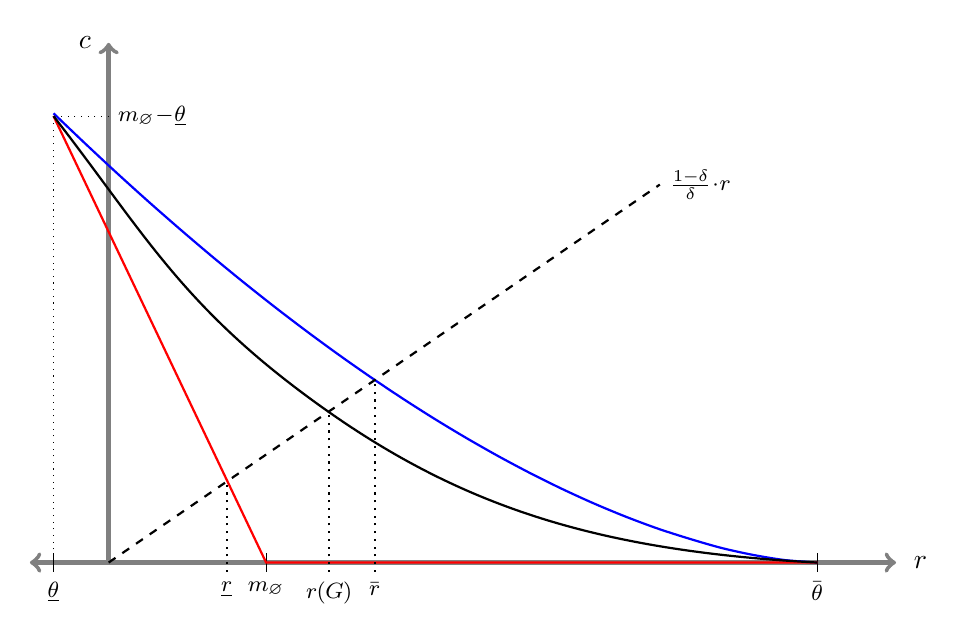
\begin{tikzpicture}[xscale=10, yscale=6]
% axis lines and labels
\draw [<->, help lines, ultra thick] (0,0) -- (1.1,0);
\draw [->, help lines, ultra thick] (0.1,0) --(.1,1.1);\node[right=3pt] at (1.1,0) {$r$};
\node[left=3pt] at (0.1, 1.1) {$c$};

% Support of F
\draw [] (1,-.02)node[below]{\footnotesize{$\bar\theta$}}--(1,.02);
\draw [] (.03,-.02) node[below]{\footnotesize{$\underline\theta$}}--(.03,.02);
\draw [dotted] (0.1, .945)node[right]{\footnotesize{$m_\varnothing -\underline\theta$}}--(0.03,.945);
\draw [dotted] (.03, 0)--(.03,.945);
\draw [] (.3,-.02) node[below]{\footnotesize{$m_\varnothing$}}--(.3,.02);

%curves
\draw[blue, domain=0.03:1,smooth,variable=\x, thick] plot ({\x},{(1-\x)^1.65});
\draw[thick, red](.03, .945)--(.3,0)--(1,0);
\draw[ thick] plot [smooth, tension=2] (0.03,.945)to [in=130, out=295](.37, .33) to [in=175, out=310](1,0);

%fixed point operator
\draw[thick, dashed] (0.1,0)--(.8,.8)node[right]{\footnotesize{$\frac{1-\delta}{\delta}\cdot r$}};

% fixed points
\draw [dotted, thick] (.38,-.02) node[below]{\footnotesize{$r(G)$}}--(.38,.32);
\draw [dotted, thick] (.25,-.02) node[below]{\footnotesize{$\underline r$}}--(.25,.172);
\draw [dotted, thick] (.438,-.02) node[below]{\footnotesize{$\bar r$}}--(.438,.39);
\end{tikzpicture}
\captionsetup{oneside,margin={0cm,0cm},justification=justified, singlelinecheck=false}
\caption{The dashed line has a slope of $(1-\delta)/\delta$. The red curve is $c_{G^\varnothing}$, the black curve is $c_G$ for some arbitrary $G\in\mathcal{G}(F)$, and the blue curve is $c_F$. The intersection of each respective curve with the dashed line represents the solu tion to the fixed point problem in \eqref{eq:2}.}
\label{fig:fix}
\end{center}
\end{figure}

\section{Stationary Equilibrium}\label{stationary}
In this section, we characterize stationary equilibrium outcomes. To that end, we make two observations that simplify our task. First,  it suffices for our purposes to consider only pure strategies because, since all players are risk neutral and the space of contracts is convex, the principal does not gain from randomizing over contracts.\footnote{Additionally, to sustain an equilibrium, we also assume that whenever the agent is indifferent between any two actions on the equilibrium path, he chooses the one that maximizes the principal's payoff.} Second,  we can restrict attention to contracts that induce the agent to accept since the agent rejecting a contract is payoff-equivalent for all players to the agent accepting a contract $\langle 0, G^\varnothing\rangle$.

\begin{definition}
\label{def:1}
\normalfont A stationary equilibrium is defined by a pair of agent-principal continuation values $(U, V)\in \mathbb{R}_+^2$ and a contract $\langle p,G\rangle\in\mathbb{R}_+\times \mathcal{G}(F)$ such that in each period and after every history:
\begin{enumerate}
    \item The agent stops searching and consumes a good of expected quality $m\in\Theta$ if and only if 
    \[
     \label{eq:os}
    \tag{OS}
    m>\delta U,
    \]
    \item The agent accepts a contract $\langle \widehat p,\widehat G\rangle\in\mathbb{R}_+\times\mathcal{G}(F)$  if and only if
    \begin{align*}
        \underbrace{\delta U+c_{\widehat G}(\delta U)-\widehat p}_{\text{payoff from accept}}&\geq \underbrace{\delta U+c_{ G^\varnothing}(\delta U)}_{\text{payoff from reject}} \\[8pt]
        \label{eq:pc}
    \tag{PC}
        \Leftrightarrow   c_{\widehat G}(\delta U)-c_{G^\varnothing}(\delta U)& \geq \widehat p,
    \end{align*}
       
\item The principal proposes contract $\langle p,G\rangle$ to maximize her profit, i.e.,
\[
\label{eq:pm}
\tag{PM}
 \langle p,G\rangle\in \argmax_{\langle \widehat p, \widehat G\rangle\in\mathbb{R}_+\times \mathcal{G}(F)}\hspace*{.2em} \widehat p+ \widehat G(\delta U) \delta V \hspace*{.5em} \text{ subject to \eqref{eq:pc}},
\]   
\item Payoffs are self-generating, i.e., 
\[
\label{eq:sga}
\tag{SG-A}
U=\delta U+c_{G}(\delta U)-p 
\] 
    and
    \[
    \label{eq:sgp}
\tag{SG-P}
V= p + G(\delta U) \delta V.
\] 
\end{enumerate}
\end{definition}


To gain some intuition of the economic forces at play, let us first consider the principal's intra-temporal trade-off\textemdash the trade-off the principal faces when proposing a contract in any given period $t\geq 1$ while holding the continuation values $(U,V)$ fixed. By selling a signal that induces a posterior-mean distribution  $\widehat G$ in period $t$, the principal can at most earn a revenue of $c_{\widehat G}(\delta U)-c_{G^\varnothing}(\delta U)$, which is captured by \eqref{eq:pc}. Additionally, she persuades the agent to continue searching in period $t$ with probability $\widehat G(\delta U)$, which is derived from \eqref{eq:os}.  The principal can extract more surplus in period $t$ by selling a more informative signal, but a more informative signal can lead the agent to stop searching with a higher probability.  Thus, the principal trades-off surplus extraction and persuasion as captured by the constrained profit maximization problem \eqref{eq:pm}.  

However, we cannot consider the intra-temporal trade-off of any given period in isolation. This is evident from the fact that the surplus the principal can extract and the probability with which she can persuade the agent to continue searching in any given period both depend on the continuation values, which are derived from the contracts the principal offers in subsequent periods. In a stationary equilibrium, the same contract must resolve the intra-temporal trade-off in each period while also taking into account how these trade-offs are inter-temporally linked. Formally, a contract $\langle p, G\rangle$ supports a stationary equilibrium if it solves \eqref{eq:pm} for given a pair of continuation values $(U,V)$, which are themselves be generated from $\langle p, G\rangle$ according to \eqref{eq:sga} and \eqref{eq:sgp}.

Our main result below establishes not only the existence of a stationary equilibrium but also that all stationary equilibria are payoff equivalent. In any stationary equilibrium, the McCall payoff $\bar u$ is generated but the agent's payoff is the same as his autarky payoff $\underline u$. The full surplus $\bar u-\underline u$ is extracted by the principal through dribs and drabs by charging a per-period price that is a (possibly small) fraction of the overall value of search.\footnote{As we show in point $(iii)$ of \autoref{prop:1}, the per-period price is strictly below $\bar u-\underline u$ for any $\delta>0$. Additionally, as $\delta\to 1$, the per-period price converges to zero while the duration of search goes to infinity. } Full surplus extraction implies that the agent searches as if he observes a fully informative signal  for free, even though his payoff is as if he observes no information.


In order to state our main result, we introduce a particular family of ``pass/fail" signals: for  $x\in\Theta$,  let $(\pi(x), \{\text{fail, pass}\})$ be given by 
 \[
\pi(\text{pass}|\theta;x)=\left\{\begin{array}{ccl}
     0 &\mbox{if} & ~~~\theta\leq  x \\
     1 &\mbox{if} & ~~~\theta> x
     \end{array}\right..
\] 
We will refer to such signals simply as $\pi(x)$ for  $x\in\Theta$, and denote the posterior-mean distribution it induces by $G^{\pi(x)}\in\mathcal{G}(F)$. Notice that both $\pi(\underline \theta)$ and $\pi(\bar \theta)$  induce $G^{\pi(\underline\theta)}=G^{\pi(\bar\theta)}=G^\varnothing$ as almost all goods pass for the former and  all goods fail for the latter. On the other hand, when $x$ is an interior point, i.e., $x\in \text{int}(\Theta)$, $\pi(x)$ induces a binary posterior-mean distribution given by 
 \[
 \label{eq:3}
\tag{3}
G^{\pi(x)}(m)=\left\{\begin{array}{ccl}
     0 &\mbox{if} & ~~~m<\mathbb{E}_F[\theta|\theta\leq  x]  \\
       F(x) &\mbox{if} &~~~ \mathbb{E}_F[\theta|\theta\leq  x]\leq m<\mathbb{E}_F[\theta|\theta>  x]  \\
     1 &\mbox{if} & ~~~m\geq \mathbb{E}_F[\theta|\theta>  x]
     \end{array}\right..
\]
We call $G^{\pi(x)}$ in \eqref{eq:3} a binary distribution as it has mass at only two values: $\mathbb{E}_F[\theta|\theta\leq  x]$ and $\mathbb{E}_F[\theta|\theta>  x]$. This family of distributions plays an important role in characterizing stationary equilibria, and we discuss its properties imminently as part of the argument for \autoref{prop:1}.
\newline 

\begin{theorem}\label{prop:1}\
A stationary equilibrium exists. A pair of agent-principal continuation values $(U, V)\in \mathbb{R}_+^2$ and a contract $\langle p,G\rangle\in\mathbb{R}_+\times \mathcal{G}(F)$ constitute a stationary equilibrium if and only if
\begin{enumerate}[$(i)$]
    \item  $U=\underline u$, 
    \item  $V=\bar u-\underline u$, 
        \item  $p=(\bar u-\underline u)\big(1-\delta F( \bar r)\big)$,
    \item $G(\underline r)=F( \bar r)$, and
    \item $c_G\geq c_{G^{\pi(\bar r)}}$ pointwise with $c_G(\underline r)= c_{G^{\pi(\bar r)}}(\underline r)$.
\end{enumerate}
\end{theorem}
\begin{proof}
Here, we provide a proof of the necessary conditions: a tuple $(p, G, U, V)$ constitutes a stationary equilibrium only if it satisfies points $(i)$-$(v)$ of the theorem. We also construct one such equilibrium, proving existence. In the \hyperref[appendix]{Appendix}, we complete the proof by showing that points $(i)$-$(v)$ are sufficient conditions.

To that end, consider a contract $\langle p, G\rangle $ along with a pair of agent-principal continuation values $(U, V)$ that constitute a stationary equilibrium. Then the contract $\langle p,G\rangle$ must  solve the constrained profit maximization problem \eqref{eq:pm}. Since the objective function in \eqref{eq:pm} is increasing in the price $\widehat p$, the constraint \eqref{eq:pc} must bind at the maximum, i.e., $p=c_{G}(\delta U)-c_{G^\varnothing}(\delta U)$. Additionally, the contract $\langle p, G\rangle $ must be consistent with the agent's self-generation condition \eqref{eq:sga} which, given the binding participation constraint, becomes   
\[
U=\delta U+c_{G^\varnothing}(\delta U).
\]
The above fixed-point problem is the same as \eqref{eq:1'} evaluated at $G^\varnothing$, and thus has a unique solution $U=u(G^\varnothing)\triangleq \underline u$  establishing point $(i)$ of the theorem.

Since the agent earns his autarky payoff $U=\underline u$ in a stationary equilibrium, from \eqref{eq:os}, he stops his search if and only if the expected quality of a good exceeds the aurarky reservation value $\underline r$. We can then rewrite the principal's profit maximization problem \eqref{eq:pm} as
\begin{align*}
&\max_{\widehat G\in\mathcal{G}(F)} \hspace*{.2em} \underbrace{c_{\widehat G}(\underline r)-c_{G^\varnothing}(\underline r)}_{=\widehat p}+\delta \widehat G(\underline r)V
\\[10pt]
\label{eq:4}
\tag{PM$'$}
=&\max_{\widehat G\in\mathcal{G}(F)}\hspace*{.2em}c_{\widehat G}(\underline r)-c_{G^\varnothing}(\underline r)+\delta\big(\partial_+ c_{\widehat G}(\underline r)+1\big)V,
\end{align*}
where the equality follows from point $(d)$ of \autoref{remark:1}. Notice that the value of $c_{\widehat G}(\underline r)$ determines the price while the slope $\partial_+c_{\widehat G}(\underline r)$ captures the probability with which the principal persuades the agent to continue searching. Since $G$ supports a stationary equilibrium, it is a solution to $\eqref{eq:4}$.

In order to solve the optimization problem in \eqref{eq:4}, we first note that the agent has only two actions upon observing a signal realization\textemdash continue searching or stop. Thus,  we can restrict attention to binary posterior-mean distributions, as stated in the lemma below. 

\begin{lemma}\label{lemma:binary}
A distribution $G\in\mathcal{G}(F)$ is a solution to  \eqref{eq:4} if and only if there exists a binary distribution $G^\dagger\in\mathcal{G}(F)$ with $\supp(G^\dagger)=\{m_1^\dagger, m_2^\dagger\}$ such that 
\begin{enumerate}[$(i)$]
    \item $m_1^\dagger\leq \underline r<m_2^\dagger$,
    \item $c_{G^\dagger}(x)\leq c_G(x)$ for all $x\in\Theta$ with equality at $x=\underline r$, 
    \item $\partial_+c_{G^\dagger}(\underline r)= \partial_+c_G(\underline r)$, and
    \item $G^\dagger$ is a solution to \eqref{eq:4}.
\end{enumerate}
\end{lemma}

% \begin{lemma}\label{lemma:binary}
% Suppose there exists $G\in\mathcal{G}(F)$ that is a solution to  \eqref{eq:4}. Then there exists a binary posterior-mean distribution $G^\dagger\in\mathcal{G}(F)$ with $\supp(G^\dagger)=\{m_1^\dagger, m_2^\dagger\}$ such that 
% \begin{enumerate}[$(i)$]
%     \item $m_1^\dagger\leq \underline r<m_2^\dagger$,
%     \item $c_{G^\dagger}(x)\leq c_G(x)$ for all $x\in\Theta$ with equality at $x=\underline r$, and
%     \item $G^\dagger$ is a solution to \eqref{eq:4}.
% \end{enumerate}
% \end{lemma}
Compared to $G$, $G^\dagger$ induces the same price (point $(ii)$ of the lemma) and the same probability of ending the search (point $(iii)$ of the lemma). Importantly, point $(i)$ of the lemma states that ``low" and the ``high" realization of the signal inducing $G^\dagger$ persuade the agent to continue and stop his search, respectively.

We turn to a graphical representation, restricting our attention to such binary distributions, to aid in solving \eqref{eq:4}. Consider two distributions $G'$ and $G''$: $c_{G'}$ is depicted by the black piece-wise linear convex curve in \autoref{fig:44a} and $c_{G''}$ is depicted by the green curve in \autoref{fig:44b} that is tangent to $c_F$ at point $x\in\Theta$. Notice
that both curves have the same slope at $\underline r$, i.e., $\partial_+c_{G'}(\underline r)=\partial_+c_{G''}(\underline r)$.  Additionally, the green curve is higher than the black curve everywhere, and strictly so at $\underline r$, i.e., $c_{G'}\leq c_{G''}$ pointwise and  $c_{G'}(\underline r)<c_{G''}(\underline r)$. Consequently, evaluating \eqref{eq:4} at $G'$ and $G''$ reveals that $G''$ yields a higher expected payoff to the principal than $G'$; both $G'$ and $G''$ persuade the agent with the same probability to continue searching but he pays a higher per-period price for $G''$.

\begin{figure}[ht]
\begin{center}
\hspace{-50mm}
\captionsetup[subfigure]{oneside,margin={1cm,-4cm}}\begin{subfigure}[t]{0.4\textwidth}
\centering
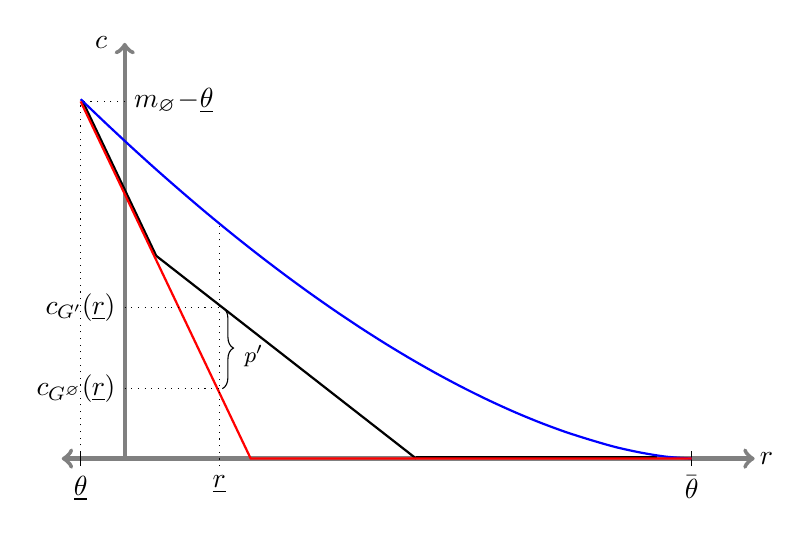
\begin{tikzpicture}[xscale=8, yscale=4.8]
% axis lines and labels
\draw [<->, help lines, ultra thick] (0,0) -- (1.1,0);
\draw [->, help lines, ultra thick] (0.1,0) --(.1,1.1);\node[right=3pt] at (1.08,0) {$r$};
\node[left=3pt] at (0.1, 1.1) {$c$};

% Support of F
\draw [] (1,-.02)node[below]{$\bar\theta$}--(1,.02);
\draw [] (.03,-.02) node[below]{$\underline\theta$}--(.03,.02);
\draw [dotted] (0.1, .945)node[right]{$m_\varnothing -\underline\theta$}--(0.03,.945);
\draw [dotted] (.03, 0)--(.03,.945);
% \draw [] (.3,-.02) node[below]{$~~m_\varnothing$}--(.3,.02);

%curves
\draw[ thick](.0327, .947)--(.15,.5365);
\draw[ thick](.562,.005)--(.945,.005);
\draw[ domain=0.15:.5629,smooth,variable=\x, thick] plot ({\x},{-1.3*(\x-.255)+.4});


%  \draw[ Green, thick](.0327, .947)--(.057,.865);
% \draw[Green, thick](.713,.01)--(.945,.01);
% \draw[Green, domain=0.05:.715,smooth,variable=\x, thick] plot ({\x},{-1.3*(\x-.255)+.607});

\draw[blue, domain=0.03:1,smooth,variable=\x, thick] plot ({\x},{(1-\x)^1.65});
\draw[thick, red](.03, .945)--(.3,0)--(1,0);
% \draw[ Green, thick] plot [smooth, tension=2] (0.03,.945)to [in=130, out=295](.37, .33) to [in=175, out=310](1,0);

%fixed point operator
% \draw[thick, dashed] (0.1,0)--(.8,.8)node[right]{$\frac{1-\delta}{\delta}$};
\draw[dotted] (0.1,0.185)node[left]{$c_{G^\varnothing}(\underline r)$}--(.255,.185);
\draw[dotted] (0.1,0.4)node[left]{$c_{G'} (\underline r)$}--(.255,.4);



%price
\draw [decorate, decoration={brace, amplitude=4pt}](0.255,0.4) -- (0.255,.185) node [black,midway,xshift=0.4 cm, yshift=-.1cm]
{\footnotesize $p'$};

%price
%\draw [decorate,decoration={brace,amplitude=15pt}]
%(0.255,0.60) -- (0.28,.185) node [black,midway,xshift=0.85cm]
%{\footnotesize $p_2$};

\draw [dotted] (.25,-.02) node[below]{$\underline r$}--(.25,.615);\end{tikzpicture}
\caption{Arbitrary binary distribution}
\label{fig:44a}
\end{subfigure} 
\hspace*{8em}
\captionsetup[subfigure]{oneside,margin={5cm,-10cm}}\begin{subfigure}[t]{0.3\textwidth}
\centering
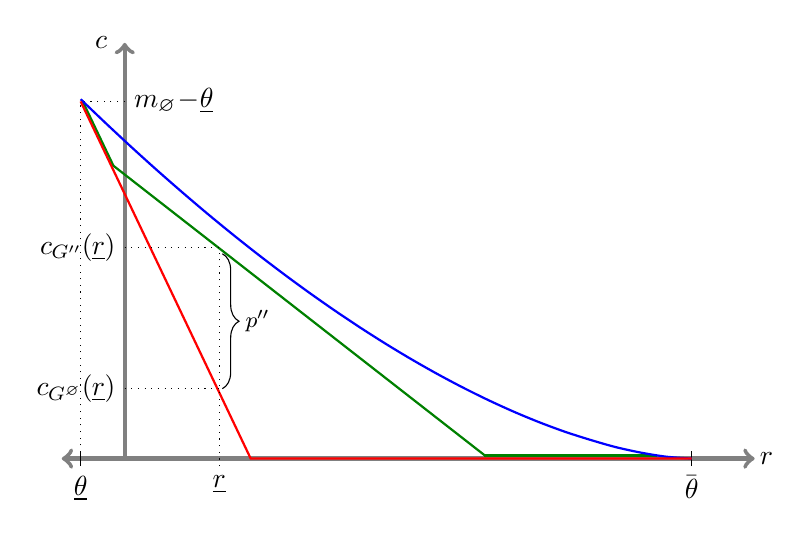
\begin{tikzpicture}[xscale=8, yscale=4.8]
% axis lines and labels
\draw [<->, help lines, ultra thick] (0,0) -- (1.1,0);
\draw [->, help lines, ultra thick] (0.1,0) --(.1,1.1);\node[right=3pt] at (1.08,0) {$r$};
\node[left=3pt] at (0.1, 1.1) {$c$};

% Support of F
\draw [] (1,-.02)node[below]{$\bar\theta$}--(1,.02);
\draw [] (.03,-.02) node[below]{$\underline\theta$}--(.03,.02);
\draw [dotted] (0.1, .945)node[right]{$m_\varnothing -\underline\theta$}--(0.03,.945);
\draw [dotted] (.03, 0)--(.03,.945);
%\draw [dotted] (.33,-.02) node[below]{$~~x$}--(.33,.5);

%curves
\draw[ Green, thick](.0327, .947)--(.082,.775);
\draw[Green, thick](.67,.008)--(.945,.008);
\draw[Green, domain=0.077:.674,smooth,variable=\x, thick] plot ({\x},{-1.3*(\x-.255)+.55});


\draw[blue, domain=0.03:1,smooth,variable=\x, thick] plot ({\x},{(1-\x)^1.65});
\draw[thick, red](.03, .945)--(.3,0)--(1,0);
% \draw[ Green, thick] plot [smooth, tension=2] (0.03,.945)to [in=130, out=295](.37, .33) to [in=175, out=310](1,0);

%fixed point operator
% \draw[thick, dashed] (0.1,0)--(.8,.8)node[right]{$\frac{1-\delta}{\delta}$};
\draw[dotted] (0.1,0.185)node[left]{$c_{G^\varnothing}(\underline r)$}--(.255,.185);
\draw[dotted] (0.1,0.558)node[left]{$ c_{G''}(\underline r)$}--(.257,.558);



%price
\draw [decorate,decoration={brace,amplitude=6pt}]
(0.255,0.542) -- (0.255,.185) node [black,midway,xshift=0.45cm]
{\footnotesize $p''$};

\draw [dotted] (.25,-.02) node[below]{$\underline r$}--(.25,.553);
\end{tikzpicture}
\vspace*{-7mm}\caption{Profit-improving binary distribution}
\label{fig:44b}
\end{subfigure}
 \captionsetup{justification=justified,singlelinecheck=false}
\caption{In both panels, the red curve is~$c_{G^\varnothing}$ and the blue curve is $c_F$. Panel (a) depicts $p'=c_{G'}(\underline r)-c_{G_\varnothing}(\underline r)$ and function $c_{G'}$ in black. Panel (b) depicts $p''=c_{G''}(\underline r)-c_{G_\varnothing}(\underline r)$ and function $c_{G''}$ in~green. $c_{G''}$ has the same slope as $c_{G'}$ at point $\underline r$ but $G'$ is a mean-preserving contraction of $G''$, which is depicted by the fact that $c_{G'}\leq c_{G''}$ pointwise. }
\label{fig:44}
\end{center}
\end{figure}

In fact, this logic shows if a binary distribution $G$ solves \eqref{eq:4}, then $c_{G}$ must be tangent to $c_F$ at some point $x\in \text{int}(\Theta)$. Such a distribution $G$ is induced by a signal that partitions $\Theta$ into sub-intervals $[\underline \theta, x]$ and $(x, \bar \theta]$. Note that, subject to relabeling ``pass" and ``fail," any such signal is equivalent to $\pi(x)$. Thus, we restrict attention to the family of binary distributions $\{G^{\pi(x)}\}_{x\in\text{int}(\Theta)}$ as defined in \eqref{eq:3}. It is easily verifiable that $c_{G^{\pi(x)}}$ is tangent to $c_F$ at $x$. The following lemma shows that it is sufficient for the optimization problem in \eqref{eq:4}  to consider a family of such binary distributions with tangency points in a compact subset of $\text{int}(\Theta)$.

\begin{lemma}\label{lemma:interval-x}
 There exists a unique point $\bar x\in(\underline r,\bar \theta)$ such that $\mathbb{E}_F[\theta|\theta\leq x]\leq \underline r<\mathbb{E}_F[\theta|\theta>x]$
if and only if $x\leq \bar x$. Furthermore, if a binary distribution $G\in\mathcal{G}(F)$  is a solution to  \eqref{eq:4}, then $G=G^{\pi(x)}$ for some $x\in[\underline r,\bar x]$.
\end{lemma}

% \begin{lemma}\label{lemma:interval-x}
%  There exists a unique point $\bar x\in(\underline r,\bar \theta)$ such that $\mathbb{E}_F[\theta|\theta\leq x]\leq \underline r<\mathbb{E}_F[\theta|\theta>x]$ 
% if and only if $x\leq \bar x$. Furthermore, if $G\in\mathcal{G}(F)$  is a solution to  \eqref{eq:4}, then there exist a point $x\in[\underline r,\bar x]$ such that $G^{\pi(x)}$ as defined in \eqref{eq:3} is also a solution to  \eqref{eq:4}. 
% \end{lemma}

The proof of \autoref{lemma:interval-x} shows two things. First, the pass/fail signal $\pi(x)$ persuades the agent  to stop his search conditional on ``pass" and to continue his search conditional on ``fail" if and only if  $x\leq \bar x$. Second, any $G^{\pi(x)}$ with $x<\underline r$ yields a strictly lower payoff than $G^{\pi(\underline r)}$, implying that no point of tangency strictly below $\underline r$ can solve \eqref{eq:4}. 

A point of tangency $x\in [\underline r, \bar x]$ pins down both the slope $\partial_+c_{G^{\pi(x)}}(\underline r)=F(x)-1$ and the price $c_{G^{\pi(x)}}(\underline r)-c_{G^\varnothing}(\underline r)$. The agent searches for the longest duration (largest slope) when $x=\bar x$, and he pays the highest per-period price when $x=\underline r$ because $c_{G^{\pi(\underline r)}}(\underline r)\geq c_{G^{\pi(x)}}(\underline r)$ for all $x$ as previously mentioned.  We can further rewrite the price  associated with distribution $G^{\pi(x)}$ as
 \begin{align*}\label{eq:price}
     c_{G^{\pi(x)}}(\underline r)-c_{G^\varnothing}(\underline r)&=c_{G^{\pi(x)}}(r(G^{\pi(x)}))+\int^{r(G^{\pi(x)})}_{\underline r}\big(1-G^{\pi(x)}(m)\big)dm-c_{G^\varnothing}(\underline r)\\[8pt]
     &=c_{G^{\pi(x)}}(r(G^{\pi(x)}))+\big(r(G^{\pi(x)})-\underline r\big)\big(1-F(x)\big)-c_{G^\varnothing}(\underline r) \notag\\[8pt]
     &=\big(u(G^{\pi(x)})-\underline u\big)\big(1-\delta F(x)\big) \tag{4},
 \end{align*}
 where $r(G^{\pi(x)})=\delta u(G^{\pi(x)})$ is the solution to \eqref{eq:2}, that is, the agent's reservation value if he were to observe $G^{\pi(x)}$ for free in every period. The first equality above follows from breaking up the integral in the definition of $c_{G^{\pi(x)}}(\underline r)$, the second equality follows by definition of $G^{\pi(x)}$ and the fact that $\mathbb{E}_F[\theta|\theta\leq x]\leq \underline r\leq  r(G^{\pi(x)})<\mathbb{E}_F[\theta|\theta>x]$,\footnote{For all $x\in [\underline r, \bar x]$, we have  $\mathbb{E}_F[\theta|\theta\leq x]\leq r(G^{\pi(x)})<\mathbb{E}_F[\theta|\theta>x]$. The first inequality follows because $\underline r\leq r(G^{\pi(x)})$ and  $\mathbb{E}_F[\theta|\theta\leq x]\leq \underline r$. The second inequality follows because if $\mathbb{E}_F[\theta|\theta>x]\leq r(G^{\pi(x)})$, then $c_{G^{\pi(x)}}(r(G^{\pi(x)}))=0$, which by \eqref{eq:2} would imply that $r(G^{\pi(x)})=0<\underline r$, yielding a contradiction.} and the last equality follows from evaluating the fixed point problems in \eqref{eq:2} at $G^{\pi(x)}$ and $G^\varnothing$.  Hence, the value of the objective function in \eqref{eq:4} is entirely determined by the point of tangency, which reduces our infinite dimensional optimization problem to a single dimensional problem:
 \begin{align*}
&\max_{x\in[\underline r, \bar x]} \hspace*{.2em} \big(u(G^{\pi(x)})-\underline u\big)\big(1-\delta F(x)\big)+\delta F(x)V.
\end{align*}

The optimization above makes clear the principal's intra-temporal trade-offs: she maximizes some convex combination of the surplus available to extract $u(G^{\pi(x)})-\underline u$ and her continuation value $V$, which is her payoff from persuading the agent to remain in the market. For $V=0$, the principal fully prioritizes surplus extraction and optimally chooses $x=\underline r$, which maximizes the per-period price. In contrast, for $V$ sufficiently large, the principal fully prioritizes persuasion and optimally chooses $x=\bar x$, which maximizes the probability the agent remains in the market.

Of course, in a stationary equilibrium, the principal's continuation value $V$ must be consistent with \eqref{eq:sgp}, i.e., 
\begin{align*}
V=&\max_{x\in[\underline r, \bar x]} \hspace*{.2em} \big(u(G^{\pi(x)})-\underline u\big)\big(1-\delta F(x)\big)+\delta F(x)V\\[8pt]
\label{eq:404}
\tag{5}
=&\max_{x\in[\underline r, \bar x]} \hspace*{.2em} u(G^{\pi(x)})-\underline u.
\end{align*}
The optimization problem in \eqref{eq:404} has two implications: First, once we impose the self-generation condition, the principal's continuation value is uniquely pinned down. Second, the self-generation condition changes the principal's incentives from some mixture of surplus extraction and persuasion into one of surplus maximization. Thus, a natural candidate for a solution to \eqref{eq:404} is to set $x$ equal to the McCall reservation value $\bar r$, which is the unique point of tangency that  generates the highest possible surplus, as stated in the following lemma. 

\begin{lemma}\label{lemma:surplus_max}
For all $x\in \Theta$ with $x\neq \bar r$,  $u(G^{\pi(x)})<u(G^{\pi(\bar r)})=\bar u$.
\end{lemma}


It remains to show that $\bar r$ lies in the desired interval $[\underline r, \bar x]$. To answer this question, consider \autoref{fig:optimal_pass_fail} which depicts $c_{G^{\pi(\bar r)}}$ as the black piece-wise convex curve that is tangent to $c_F$ at $x=\bar r$. The kinks occur at the support points $m_1^*=\mathbb{E}_F[\theta|\theta\leq x=\bar r]$ and $m_2^*=\mathbb{E}_F[\theta|\theta>x=\bar r]$. It is clear from the figure that $m_1^*<\underline r<m_2^*$, implying by \autoref{lemma:interval-x} that $\bar r\in (\underline r, \bar x)$. Indeed, this observation is not a coincidence but a general property as stated in the following lemma. The proof shows that if $\bar r\notin (\underline r, \bar x)$, then the agent would have zero WTP for any signal the principal could offer, which cannot occur in non-trivial settings that satisfy \hyperref[ass:1]{\Cref{ass:1}}.  

 \begin{lemma}\ 
\label{lemma:2} The McCall reservation value $\bar r$ lies in the open interval $(\underline r, \bar x)$. In particular, $G^{\pi(\bar r)}(m)=F(\bar r)$ for all $m\in [\underline r, \bar r]$.
\end{lemma}\

\begin{figure}[ht]
\begin{center}
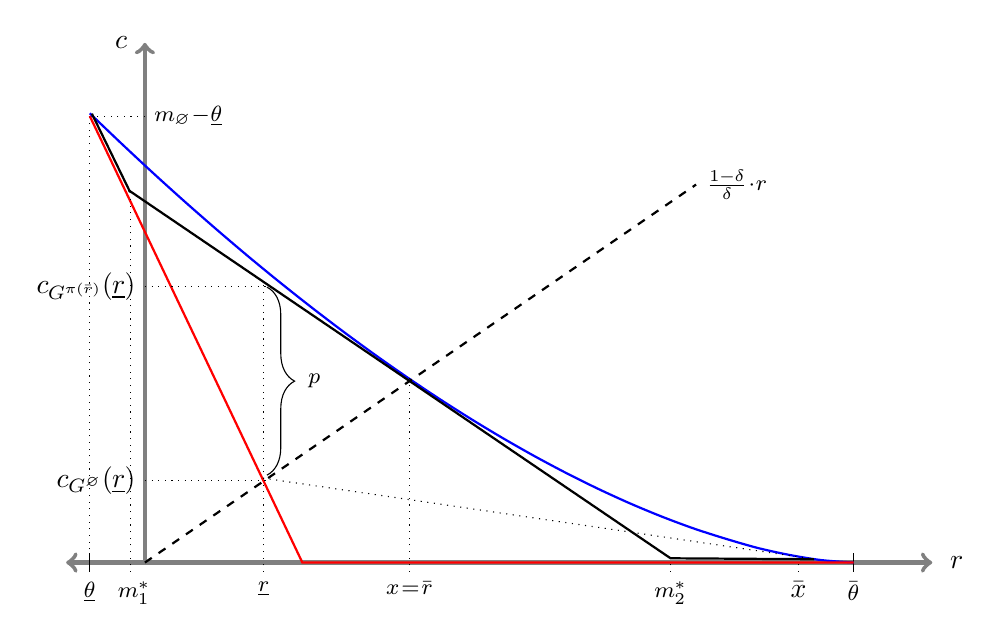
\begin{tikzpicture}[xscale=10, yscale=6]
% axis lines and labels
\draw [<->, help lines, ultra thick] (0,0) -- (1.1,0);
\draw [->, help lines, ultra thick] (0.1,0) --(.1,1.1);\node[right=3pt] at (1.1,0) {$r$};
\node[left=3pt] at (0.1, 1.1) {$c$};

% Support of F
\draw [] (1,-.02)node[below]{\footnotesize{$\bar\theta$}}--(1,.02);
\draw [] (.03,-.02) node[below]{\footnotesize{$\underline\theta$}}--(.03,.02);
\draw [dotted] (0.1, .945)node[right]{\footnotesize{$m_\varnothing -\underline\theta$}}--(0.03,.945);
\draw [dotted] (.03, 0)--(.03,.945);


%curves
\draw[blue, domain=0.03:1,smooth,variable=\x, thick] plot ({\x},{(1-\x)^1.65});
\draw[thick, red](.03, .945)--(.3,0)--(1,0);
%\draw[ thick](.0327, .95)--(.18,.435)--(.55,.38)--(.75,.009);
\draw[domain=0.0799:.768,smooth,variable=\x, thick] plot ({\x},{-1.131895*(\x-.44)+.3798});
\draw[ thick](.0327, .95)--(.0813,.784);
\draw[ thick](.7675,.009)--(.95,.007);

%support of G^*
\draw[dotted](.0813,-0.02)node[below]{\footnotesize{~$m^*_1$}}--(.0813,.784);
\draw[ dotted](.7675,-0.02)node[below]{\footnotesize{$m^*_2$}}--(.7675,0.0);
%fixed point operator
\draw[thick, dashed] (0.1,0)--(.8,.8)node[right]{\footnotesize{$\frac{1-\delta}{\delta}\cdot r$}};

% fixed points
\draw [dotted] (.251,-.02) node[below]{\footnotesize{$\underline r$}}--(.251,.59);
\draw [dotted] (.436,-.02) node[below]{\footnotesize{$x=\bar r$}}--(.436,.39);

 %price
\draw [decorate,decoration={brace,amplitude=10pt}]
 (0.255,0.583) -- (0.255,.185) node [black,midway,xshift=0.6cm]
 {\footnotesize $p$};

 \draw[dotted] (0.1,0.174)node[left]{$c_{G^\varnothing}(\underline r)$}--(.255,.174);
\draw[dotted] (0.1,0.585)node[left]{$c_{G^{\pi(\bar r)}} (\underline r)$}--(.255,.585);

% \bar x stuff

\draw[domain=0.25:.95,smooth,variable=\x, dotted] plot ({\x},{-.245*\x+.24});
% \draw[ Green,  thick](.0327, .95)--(.25,.185);
% \draw[ Green,  thick](.95,.0)--(1,.0);

%fixed point operator
% \draw[thick, dashed] (0.1,0)--(.8,.8)node[right]{$\frac{1-\delta}{\delta}$};

\draw [dotted] (.93,-.02) node[below]{$\bar x$}--(.93,.02);

\end{tikzpicture}
\captionsetup{justification=justified,singlelinecheck=false}
\caption{The red curve is $c_{G^\varnothing}$, the blue curve is $c_F$, and the black curve is $c_{G^{\pi(\bar r)}}$. Note that the support points satisfy $m_1^*<\underline r<\bar r<m_2^*< \bar x$.}
\label{fig:optimal_pass_fail}
\end{center}
\end{figure}

 Thus, the unique solution to \eqref{eq:404} is at $x=\bar r$, which yields $V=\bar u-\underline u$, establishing point $(ii)$ of the theorem. Furthermore, it implies that   $G^{\pi(\bar r)}$ is the unique binary distribution that solves \eqref{eq:4}.
 
 So far, we have shown that if the tuple $(p, G, U, V)$ constitutes a stationary equilibrium, then the agent's continuation value is $U=\underline u$, the principal's continuation value is $V=\bar u-\underline u$, the price is $p=c_G(\underline r)-c_{G^\varnothing}(\underline r)$, and the posterior-mean distribution $G$ is a solution to \eqref{eq:4}.  By point $(ii)$ of \autoref{lemma:binary}, $c_{G^{\pi(\bar r)}}(x)\leq c_G(x)$ for all $x\in\Theta$ with equality at $x=\underline r$.
This implies that the price is \begin{align*}
    p&=c_G(\underline r)-c_{G^\varnothing}(\underline r)\\[6pt]
    &=c_{G^{\pi(\bar r)}}(\underline r)-c_{G^\varnothing}(\underline r)\\[6pt]
    &=(\bar u-\underline u)(1-\delta F(\bar r)),
\end{align*} 
where the last equality follows from \eqref{eq:price}. This establishes point $(iii)$ of the theorem. Furthermore, by point $(iii)$ of \autoref{lemma:binary}, $\partial_+c_G(\underline r)=\partial_+c_{G^{\pi(\bar r)}}(\underline r)$, which by point $(d)$ of \autoref{remark:1} is equivalent to $G(\underline r)=G^{\pi(\bar r)}(\underline r)=F(\bar r)$, establishing point $(iv)$ of the theorem. Finally, by point $(ii)$ of \autoref{lemma:binary}, $c_{G^{\pi(\bar r)}}\leq c_G$ pointwise with equality at $\underline r$, establishing point $(v)$ of the theorem.  
\end{proof}\\



From the statement of \autoref{prop:1}, it is clear that the price and the continuation values in a stationary equilibrium are uniquely pinned down. However, there are  an uncountable number of posterior-mean distributions that can support a stationary equilibrium. For example, consider a lower-censorship signal that  reveals a good's quality if it exceeds $\bar r$ and pools all goods whose quality lies below $\bar r$ by labeling them as ``fail." This signal induces the distribution $G^{LC}$ given by 
\[
G^{LC}(m)=\left\{\begin{array}{ccl}
   0 &\mbox{if} &~~~ m<\mathbb{E}_F[\theta|\theta\leq \bar   r]  \\
       F(\bar r) &\mbox{if} &~~~ \mathbb{E}_F[\theta|\theta\leq \bar r]\leq m<  \bar r  \\
     F(m) &\mbox{if} & ~~~m\geq \bar r
     \end{array}\right. .
\]
Note that this lower-censorship signal is Blackwell more informative than the pass/fail signal that induces $G^{\pi(\bar r)}$. Hence, $G^{\pi(\bar r)}$ is a mean-preserving contraction of $G^{LC}$---i.e. $c_{G^{\pi(\bar r)}}\leq c_{G^{LC}}$ pointwise as can be seen in \autoref{fig:optdist}---and $G^{LC}$ also supports a stationary equilibrium as it satisfies points $(iv)$ and $(v)$ of \autoref{prop:1}.
 
%  \begin{figure}[ht]
% \begin{center}
% \begin{subfigure}{0.3\textwidth}
% \begin{tikzpicture}[scale=1]
% \draw[->, thick] (0,0) -- (4.5,0);
% \draw[->, thick] (0.7,0) -- (0.7,4.5) ;
% % axis label
% \draw [] (4,-.02)node[below]{\footnotesize{$\bar\theta$}}--(4,.02);
% \draw [] (0,-.02)node[below]{\footnotesize{$\underline\theta$}}--(0,.02);
% \draw [] (2,-.02)node[below]{\footnotesize{$\underline r$}}--(2,.02);
% \draw [] (2.75,-.02)node[below]{\footnotesize{$\bar r$}}--(2.75,.02);
% \draw [] (3.25,-.02)node[below]{\footnotesize{$m_2$}}--(3.25,.02);
% \draw [] (1.25,-.02)node[below]{\footnotesize{$m_1$}}--(1.25,.02);
% \draw [] (0.68,1.25)node[left]{\footnotesize{$F( \bar r)$}}--(0.72,1.25);

% \draw (0.7,4)node[anchor=east]{1};
% % F
% \draw[thick, dashed]  (0,0) to [bend right=40](4,4);
% \draw[ultra thick, red]  (1.25,1.25) to (3.25, 1.25);
% \draw[ultra thick, red]  (0,0) to (1.25, 0);
% \draw[ultra thick, red]  (3.25,4) to (4, 4);
% \end{tikzpicture}	
% \caption{$G^{\pi(\bar r)}$ induced by optimal pass/fail.}
% \label{fig:passfail}
% \end{subfigure}\hspace{0.15\textwidth}
% \begin{subfigure}{0.3\textwidth}
% \begin{tikzpicture}[scale=1]
% \draw[->, thick] (0,0) -- (4.5,0);
% \draw[->, thick] (0.7,0) -- (0.7,4.5) ;
% % axis label
% \draw [] (4,-.02)node[below]{\footnotesize{$\bar\theta$}}--(4,.02);
% \draw [] (0,-.02)node[below]{\footnotesize{$\underline\theta$}}--(0,.02);
% \draw [] (2,-.02)node[below]{\footnotesize{$\underline r$}}--(2,.02);
% \draw [] (2.75,-.02)node[below]{\footnotesize{$\bar r$}}--(2.75,.02);
% \draw [] (1.25,-.02)node[below]{\footnotesize{$m_1$}}--(1.25,.02);
% \draw [] (0.68,1.25)node[left]{\footnotesize{$F( \bar r)$}}--(0.72,1.25);

% \draw (0.7,4)node[anchor=east]{1};

% % F and G
% \draw[thick, dashed]  (0,0) to [bend right=40](4,4);
% \draw[ultra thick, red]  (1.25,1.25) to (2.75, 1.25);
% \draw[ultra thick, red]  (0,0) to (1.25, 0);
% % \draw[thick, red]  (2.75, 1.25) to [bend right=19](4,4);
% \draw[ultra thick, red]  plot [smooth, tension=2](2.75, 1.25) to [in=262,  out=45](4,4);
% \end{tikzpicture}	
% \caption{$G^{LC}$ induced by optimal lower-censorship.}
% \label{fig:lowercensor}
% \end{subfigure}
% \captionsetup{oneside,margin={1cm,0cm},justification=raggedright,singlelinecheck=false}
% \caption{The dashed curve corresponds to an arbitrary~prior~distribution~$F$, the red curves correspond to two different posterior-mean~distributions~that can support a stationary equilibrium, and $m_1\triangleq\mathbb{E}_F[\theta|\theta\leq \bar r]$~and~$m_2\triangleq\mathbb{E}_F[\theta|\theta> \bar r]$. Note that both distributions are constant on $[\underline r, \bar r]$. }
% \label{fig:optdist}
% \end{center}
% \end{figure}

\begin{figure}[ht]
\begin{center}
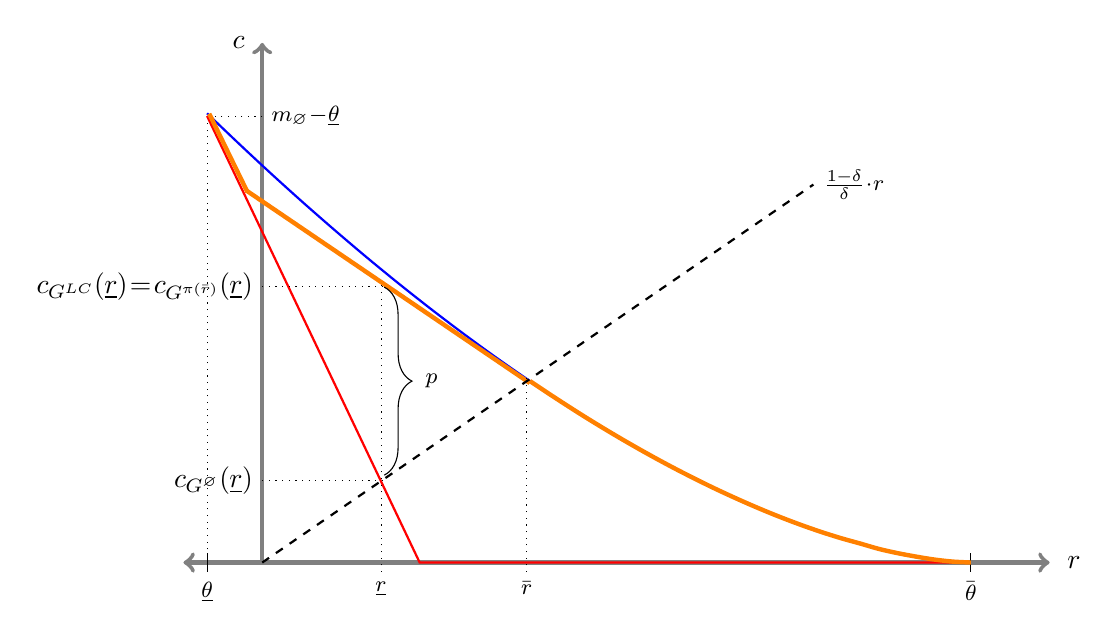
\begin{tikzpicture}[xscale=10, yscale=6]
% axis lines and labels
\draw [<->, help lines, ultra thick] (0,0) -- (1.1,0);
\draw [->, help lines, ultra thick] (0.1,0) --(.1,1.1);\node[right=3pt] at (1.1,0) {$r$};
\node[left=3pt] at (0.1, 1.1) {$c$};

% Support of F
\draw [] (1,-.02)node[below]{\footnotesize{$\bar\theta$}}--(1,.02);
\draw [] (.03,-.02) node[below]{\footnotesize{$\underline\theta$}}--(.03,.02);
\draw [dotted] (0.1, .945)node[right]{\footnotesize{$m_\varnothing -\underline\theta$}}--(0.03,.945);
\draw [dotted] (.03, 0)--(.03,.945);


%curves
\draw[blue, domain=0.03:1,smooth,variable=\x, thick] plot ({\x},{(1-\x)^1.65});
\draw[thick, red](.03, .945)--(.3,0)--(1,0);
%\draw[ thick](.0327, .95)--(.18,.435)--(.55,.38)--(.75,.009);
\draw[domain=0.0799:.44,smooth,variable=\x, orange, ultra thick] plot ({\x},{-1.131895*(\x-.44)+.3798});
\draw[ orange, ultra thick](.0327, .95)--(.0813,.784);
\draw[orange, domain=0.44:1,smooth,variable=\x, ultra thick] plot ({\x},{(1-\x)^1.65});

%support of G^*
%\draw[dotted](.0813,-0.02)node[below]{\footnotesize{~$m^*_1$}}--(.0813,.784);
%\draw[ dotted](.7675,-0.02)node[below]{\footnotesize{$m^*_2$}}--(.7675,0.0);
%fixed point operator
\draw[thick, dashed] (0.1,0)--(.8,.8)node[right]{\footnotesize{$\frac{1-\delta}{\delta}\cdot r$}};

% fixed points
\draw [dotted] (.251,-.02) node[below]{\footnotesize{$\underline r$}}--(.251,.59);
\draw [dotted] (.436,-.02) node[below]{\footnotesize{$\bar r$}}--(.436,.39);

 %price
\draw [decorate,decoration={brace,amplitude=10pt}]
 (0.255,0.583) -- (0.255,.185) node [black,midway,xshift=0.6cm]
 {\footnotesize $p$};

 \draw[dotted] (0.1,0.174)node[left]{$c_{G^\varnothing}(\underline r)$}--(.255,.174);
\draw[dotted] (0.1,0.585)node[left]{$c_{G^{LC}} (\underline r)=c_{G^{\pi(\bar r)}} (\underline r)$}--(.255,.585);

% \bar x stuff

%\draw[domain=0.25:.95,smooth,variable=\x, dotted] plot ({\x},{-.245*\x+.24});
% \draw[ Green,  thick](.0327, .95)--(.25,.185);
% \draw[ Green,  thick](.95,.0)--(1,.0);

%fixed point operator
% \draw[thick, dashed] (0.1,0)--(.8,.8)node[right]{$\frac{1-\delta}{\delta}$};

%\draw [dotted] (.93,-.02) node[below]{$\bar x$}--(.93,.02);

\end{tikzpicture}
\captionsetup{justification=raggedright,singlelinecheck=false}
\caption{The red curve is~$c_{G^\varnothing}$, the~blue~curve~is~$c_F$,~and~the~orange~curve~is~$c_{G^{LC}}$. $c_{G^{LC}}(y)=c_{G^{\pi(\bar r)}}(y)$ for all $y\in [\underline \theta,\bar r]\cup\{\bar\theta\}$, and $c_{G^{LC}}(y)>c_{G^{\pi(\bar r)}}(y)$ for all $y\in (\bar r,\bar \theta).$ }
\label{fig:optdist}
\end{center}
\end{figure}
 

Despite the multitude of equilibrium distributions, all of them have the same distribution on $[\underline r,  \bar r]$. Thus, all equilibrium signals induce the same search behavior in the agent. 

\begin{corollary}
\label{cor:1}
If a contract $\langle p, G\rangle\in\mathbb{R}_+\times\mathcal{G}(F)$ supports a stationary equilibrium, then $G(m)=F(\bar r)$ for all  $m\in [\underline r, \bar r]$.
\end{corollary}

\autoref{prop:1} characterizes the set of signals that arise in a stationary equilibrium and \autoref{cor:1} shows that all of them are equally valuable to the agent. Additionally, the principal is indifferent across all the equilibrium signals that she can generate, which precludes a unique prediction. Of course, the principal could have preferences over the set of equilibrium signals, for example, if signal production is costly. If the cost of a signal is increasing in the Blackwell order, i.e.,  $(\pi, S)$ is more costly than  $(\pi', S')$ if $(\pi, S)$ is Blackwell more informative than $(\pi', S')$, then the binary ``pass/fail" signal is the cheapest from the set of signals satisfying \autoref{prop:1}. If the cost of a signal is instead increasing in the number of realizations in its support, then the equilibrium signal is uniquely pinned down by the binary ``pass/fail" signal. This is because any signal with support over just one realization is uninformative, so any contract accepted by the agent in a stationary equilibrium must have support over at least two possible realizations.




\section{Public Signals}\label{public}

Thus far, we have assumed that the agent is  solely dependent on the principal to learn about a good's quality. However, there are settings in which public information is available about the sampled good. In this section,
we consider an agent who learns about a good's quality both by observing 
a signal $(\xi, Z)$, where $Z$ is a compact set of signal realizations and $\xi:\Theta\to \Delta (Z)$, and by contracting with the principal. We refer to $(\xi, Z)$ as a public signal because its realizations are observed by both the principal and the agent for free. Without loss of generality, we assume that $\xi$ has full support on $Z$. Additionally, for ease of exposition, we assume that the posterior beliefs conditional on observing any $z\in Z$ are atomless.

We amend the timing of events within each period $t\geq 1$ as follows: First, the agent samples a good of quality $\theta_t$ which is unobserved by  the agent and the principal. However, both observe a public signal realization $z_t\in Z$ which is distributed according to $\xi(\theta_t)$. The principal then offers a  contract $\langle p_t, (\pi_t, S_t)\rangle$ which the agent either accepts or rejects. If the agent accepts the contract $(a_t=1)$, he pays $p_t$ and observes an additional signal realization $s_t\in S$ distributed according to $\pi_t(\theta_t)$. If the agent instead rejects the contract $(a_t=0)$, he pays nothing and observes no additional signal. Finally, the agent decides whether to consume the sampled good and stop searching $(d_t=1)$ or to continue searching $(d_t=0)$. \autoref{fig:timing2} depicts the amended timing of events. 

\begin{figure}[ht]
\centering 
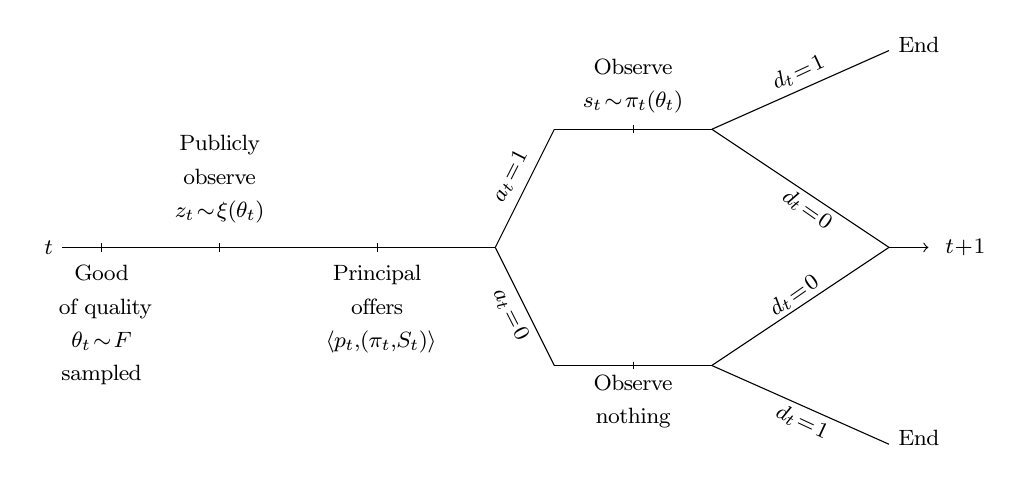
\begin{tikzpicture}[scale=0.5]
\tikzset{
    position label/.style={
             text depth = 1ex
    }
}
    \foreach \x in {-8, -5, -1}
      \draw (\x cm,3pt) -- (\x cm,-3pt);
\draw[-] (-9,0) node[left]{\footnotesize{ $t$}}--(2,0);
\draw[-] (2,0)--(3.5,3);
\draw[-] (2,0)--(3.5,-3);
\draw[-] (3.5,-3)--(7.5,-3);
\draw[-] (3.5,3)--(7.5,3);
\draw[-] (7.5,-3)--(12,0);
\draw[-] (7.5,-3)--(12,-5);
\draw[-] (7.5,3)--(12,5);
\draw[-] (7.5,3)--(12,0);
\draw[->] (12,0)--(13,0)node[right]{\footnotesize{ ${t+1}$}};

\node [position label, align=center, below=3pt] (fend) at (-8,0) {\footnotesize{Good} \\ \footnotesize{ of quality}\\ \footnotesize{$\theta_t\sim F$}\\ \footnotesize{sampled}};
\node [position label, align=center, above=3pt] (fend) at (-5,0) {\footnotesize{Publicly} \\  \footnotesize{observe}\\ \footnotesize{$z_t\sim \xi(\theta_t)$}};
\node [position label, align=center, below=3pt] (fend) at (-1,0) {\footnotesize{Principal} \\ \footnotesize{offers}\\ \footnotesize{ $\langle p_t, (\pi_t, S_t)\rangle$}};
\node [position label, rotate=63, align=center, above] (fend) at (3,1.5) {\footnotesize{$a_t=1$}};
\node [position label, rotate=297, align=center, below] (fend) at (2.8,-1.5) {\footnotesize{$a_t=0$}};


\draw[](5.5,3.1)--(5.5,2.9);
\draw[](5.5,-3.1)--(5.5,-2.9);


\node [position label, align=center, above] (fend) at (5.5,3) {\footnotesize{Observe}\\ \footnotesize{$s_t\sim\pi_t(\theta_t)$}};
\node [position label, align=center, below] (fend) at (5.5,-3) {\footnotesize{Observe}\\ \footnotesize{nothing}};

% \draw[](13,3.1)--(13,2.9);
% \draw[](13,-3.1)--(13,-2.9);
\node [position label, align=center, right] (fend) at (12,5) {\footnotesize{End}};
\node [position label, align=center, right] (fend) at (12,-5) {\footnotesize{End}};

\node [position label, rotate=335, align=center, below] (fend) at (10,-4) {\footnotesize{$d_t=1$}};
\node [position label, rotate=35, align=center, above] (fend) at (10,-1.8) {\footnotesize{$d_t=0$}};

\node [position label, rotate=25, align=center, above] (fend) at (10,3.8) {\footnotesize{$d_t=1$}};
\node [position label, rotate=325, align=center, below] (fend) at (10.2,1.35) {\footnotesize{$d_t=0$}};
  \end{tikzpicture}
  \caption{Timing of events with a public signal}
  \label{fig:timing2}
\end{figure} 

Consider first the case of autarky in which the agent can only observe a realization of the public signal $(\xi, Z)$. His induced posterior-mean distribution is $G^\xi\in\mathcal{G}(F)$ and his expected payoff in the search market is $u(G^\xi)$, which is the solution to \eqref{eq:1'} evaluated at $G^\xi$. Note that $u(G^\xi)\geq \underline u$, i.e., the agent's autarky payoff improves in the current setting since he has access to a free signal. Therefore, the full surplus that can be generated is now $\bar u - u(G^\xi).$

Next, consider the case in which agent can observe the public signal followed by a second signal. Given a public signal realization $z\in Z$, the agent updates his belief from his prior $F$ to an interim belief $F_{z}^{\xi}$. When the agent further updates his belief based on the second signal, $F^\xi_z$ serves as his new ``prior."  Thus, the set of posterior-mean distributions that can be induced through a second signal is the set of mean-preserving contractions of $F^\xi_z$, i.e., $\mathcal{G}(F^\xi_z)$. For example, a fully informative second signal induces $F^{\xi}_z$ itself, whereas an uninformative  second signal induces the degenerate distribution
\[
G^\varnothing_z(m)=\left\{\begin{array}{ccl}
     0 &\mbox{if} & m<\mathbb{E}_{F^\xi_z}[\theta]  \\
     1 &\mbox{if} & m\geq \mathbb{E}_{F^\xi_z}[\theta]  
     \end{array}\right..
\]


Therefore, following a public signal realization $z\in Z$, the principal can propose any contract of the form $\langle p, G\rangle\in\mathbb{R}_+\times \mathcal{G}(F^\xi_z)$. Our goal is to characterize stationary equilibrium outcomes. However, we must first update the conditions  for a stationary equilibrium given in \autoref{def:1} to account for the presence of a public signal.  

\begin{definition}
    \label{def:2}
    \normalfont Given a public signal $(\xi, Z)$, a stationary equilibrium  is defined by a pair of  continuation values $(U, V)\in \mathbb{R}_+^2$ and a family of  contracts $\{\langle p_z,G_z\rangle\}_{z\in Z}$ with $\langle p_z, G_z\rangle\in\mathbb{R}_+\times \mathcal{G}(F^\xi_z)$ for each $z\in Z$ such that in each period and after every history:
    \begin{enumerate}
    \item The agent stops searching and consumes a good of expected quality $m\in \Theta$ if and only if $m>\delta U$, i.e.,  \eqref{eq:os} holds,  

    \item Given a public signal realization $z$, the agent accepts  $\langle \widehat p,\widehat G\rangle\in\mathbb{R}_+\times\mathcal{G}(F^\xi_z)$  if and only if
    \begin{align*}
          \label{eq:pc2}
    \tag{PC$^\xi_z$}
           c_{\widehat G}(\delta U)-c_{G_z^\varnothing}(\delta U) \geq \widehat p,
    \end{align*}
       
\item Given a public signal realization $z$, the principal proposes $\langle p_z,G_z\rangle$ to maximize her profit, i.e.,
\[
\label{eq:pm2}
\tag{PM$^\xi_z$}
 \langle p_z,G_z\rangle\in \argmax_{\langle \widehat p, \widehat G\rangle\in\mathbb{R}_+\times \mathcal{G}(F^\xi_z)}\hspace*{.2em} \widehat p+ \widehat G(\delta U) \delta V \hspace*{.5em} \text{ subject to \eqref{eq:pc2}},
\]   
\item Payoffs are self-generating, i.e.,
\[
\label{eq:sga2}
\tag{SG-A$^\xi$}
U=\int_Z\Big(\delta U+c_{G_z}(\delta U)-p_z\Big) \xi(dz)
\] 
    and
    \[
    \label{eq:sgp2}
\tag{SG-P$^\xi$}
V= \int_Z\Big(p_z + G_z(\delta U) \delta V\Big)\xi(dz).
\] 
\end{enumerate}
\end{definition} 

Compared to \autoref{def:1}, the sequential rationality conditions in \autoref{def:2} must hold following every public signal realization $z\in Z$, which is captured by the $z$-dependent participation constraint \eqref{eq:pc2} and profit maximization problem \eqref{eq:pm2}. In contrast, the self-generation conditions \eqref{eq:sga2} and \eqref{eq:sgp2} hold only in expectation.

In order to state our main result of this section, we must first introduce some notation. Let $r^\xi\triangleq r(G^\xi)$ be the agent's reservation value in autarky when his only source of information is the pubic signal. Given a public signal realization $z\in Z$, we denote the lower and upper bounds on the support of $F^\xi_z$ by $\underline \theta_z\triangleq\inf \hspace*{.2em} \supp(F^\xi_z)$ and $\bar \theta_z\triangleq\sup \hspace*{.3em}\supp(F^\xi_z)$ respectively. For some $k\geq 0$, let
\[
Z_A(k)\triangleq\{z\in Z:r^\xi \hspace*{.1em} < \hspace*{.1em}\underline \theta_z<\bar r-k\}.
\]
In the case that $r^\xi\in [\underline\theta_z, \bar\theta_z]$, let 
$\bar x_z\triangleq\sup\{x\in [\underline\theta_z, \bar\theta_z]:\mathbb{E}_{F_z^\xi}[\theta|\theta\leq x]\leq r^\xi\}$, and for some $k\geq 0$, let 
\[
Z_B(k)\triangleq\big\{z\in Z:r^\xi\in [\underline \theta_z ,\bar\theta_z]\hspace*{.1em} \wedge \hspace*{.1em}\bar x_z\hspace*{.1em} < \min\{\bar \theta_z, \hspace*{.1em}\bar r-k\}\big\}.
\]
Note that $Z_A(k)$ and $Z_B(k)$ could be empty. Finally, we define  the function $\Phi:\mathbb{R}_+\to \mathbb{R}$ by
       \small{\begin{align*}
        \label{eq:5}
        \tag{6}
\Phi(k)\triangleq \int_{\bar r-k}^{\bar r}F(m)dm+\int_{Z_A(k)}\int_{\underline\theta_z}^{\bar r-k}F^\xi_z(m)dm \xi(dz)+\int_{Z_B(k)}\int_{\bar x_z}^{\bar r -k}\big(F^\xi_z(m)-F^\xi_z(\bar x_z)\big)dm\xi(dz). 
        \end{align*}} %%
        
       \normalsize 
\noindent We provide a detailed discussion of  $Z_A(\cdot)$, $Z_B(\cdot)$, and $\Phi(\cdot)$ following the statement of the following theorem.

\begin{theorem}
\label{prop:2}
    For any public signal $(\xi, Z)$, a stationary equilibrium exists. Furthermore, in any stationary equilibrium, 
    \begin{enumerate}[$(i)$]
        \item $U=u(G^\xi)$ and
        \item $V=\bar u-u(G^\xi)-\displaystyle\frac{k^*}{\delta}$, where $k^*\in [0, \bar r-r^\xi]$ is the unique solution to the fixed point 
        \[
        k=\delta\Phi(k).
        \]
    \end{enumerate}
\end{theorem}

\autoref{prop:2} establishes that for any given public signal, a stationary equilibrium exists and that all stationary equilibria are payoff equivalent. The agent gets his autarky payoff $u(G^\xi)$, which is now (potentially strictly) higher than $\underline u$, whereas the principal's payoff may be (potentially strictly) lower than the maximal surplus that she could feasibly extract $\bar u-u(G^\xi)$. In other words, introducing a free and public signal may lead to an inefficient outcome with $k^*/\delta$ measuring the total welfare loss in equilibrium.

The maximum surplus is created if and only if the agent stops his search for a  good whose quality exceeds the McCall reservation value $\bar r$. However, because the agent earns his autarky payoff in a stationary equilibrium, he will stop his search if and only if a good's expected quality exceeds the autarky reservation value $r^\xi$. Therefore, whenever $r^\xi<\bar r$, the principal can create (and extract) additional surplus if she can persuade the agent to search as if his reservation value is higher than $r^\xi$. The proof of \autoref{prop:2} demonstrates the principal can induce a reservation value of $x_z\in[r^\xi, \bar r]$ following a public signal realization $z\in Z$ if and only if the pass/fail signal $\pi(x_z)$---which recall fails a good  if its true quality is $\theta\leq x_z$ and passes it otherwise---persuades the agent to continue searching when he observes a ``fail" and to stop searching when he observes a ``pass," i.e., $\mathbb{E}_{F_z^\xi}[\theta|\theta\leq x_z]\leq r^\xi<\mathbb{E}_{F_z^\xi}[\theta|\theta> x_z]$ respectively.\footnote{As in the case without a public signal, it is easy to see that $\mathbb{E}_{F_z^\xi}[\theta|\theta> x_z]>r^\xi$ holds for any $x_z\geq r^\xi$.}

To understand when the public signal causes an efficiency loss, suppose for some $k\in [0, \bar r-r^\xi]$, the principal seeks to induce a reservation value of $x_z=\bar r - k$ for all  $z\in Z$ by offering the pass/fail signal $\pi(\bar r-k)$. The loss of surplus stemming from the difference between the induced reservation value $\bar r-k$ and the McCall reservation value $\bar r$ is characterized by $\Phi(k).$  To see why, notice that the decrease in surplus from inducing $\bar r-k$ instead of $\bar r $ given a public signal realization $z\in Z$ is captured by 
\[
\mathbb{E}_{F^\xi_z}[\max\{\theta, \bar r\}]-\mathbb{E}_{F^\xi_z}[\max\{\theta, \bar r-k\}]=\int^{\bar r}_{\bar r-k}F^\xi_z(m)dm. 
\]
 which in expectation yields the first term in \eqref{eq:5} after noting that $\mathbb{E}_{\xi}[F_z^\xi]=F$ by Bayes-plausibility. 

However, the first term in \eqref{eq:5} captures the change in the total surplus assuming the principal can induce $\bar r-k$ for all realizations of the public signal. Yet, there are two cases when the principal cannot induce the desired reservation value following a public signal realization $z\in Z$. First, suppose the agent observes a public signal realization $z\in Z$ such that $r^\xi<\underline \theta_z$. In this case, no additional information can affect the agent's search as he already observes conclusive evidence that the quality of the sampled good is above his autarky reservation value, leading him to terminate his search. However, when $\underline\theta_z<\bar r-k$, the principal would like the agent to continue searching when the sampled good's quality lies in the interval $[\underline\theta_z, \bar r-k]$. This is precisely the case when $z\in Z_A(k)$, and the additional surplus loss is captured by 
 \[
\int_{\underline \theta_z}^{\bar r-k}\big(\bar r-k-m\big)dF_Z^\xi(m)=\int_{\underline \theta_z}^{\bar r-k}F^\xi_z(m)dm,
 \]
 which in expectation yields the second term in \eqref{eq:5}.


Second, suppose the agent observes a public signal realization $z\in Z$ such that $r^\xi\in [\underline \theta_z ,\bar\theta_z]$. In this case, the agent's decision to either continue or stop his search depends on the additional information the principal provides. In particular, by definition of $\bar x_z$, the agent is persuaded to continue his search when he observes a ``fail" from a pass/fail signal $\pi(x_z)$ with $x_z\leq \bar x_z$. Notice that  $\bar x_z=\bar \theta_z$ implies the agent continues searching without additional information (i.e., $\mathbb{E}_{F_z^\xi}[\theta]\leq r^\xi$), whereas $\bar x_z<\bar \theta_z$ implies the agent stops searching without additional information (i.e., $\mathbb{E}_{F_z^\xi}[\theta]> r^\xi$).
 Thus, if $\bar x_z<\min\{\bar \theta_z, \bar r-k\}$, the principal would like the agent to continue searching when the sampled good's quality lies in the interval $[\underline\theta_z, \bar r-k]$, but the agent would stop his search with probability one if the principal offers him the pass/fail signal $\pi(\bar r-k)$. This is precisely the case when $z\in Z_B(k)$. Intuitively, a public signal realization $z\in Z_B(k)$ induces an interim posterior belief $F_z^\xi$ that places more mass on the interval $[r^\xi, \bar r-k]$ than it does on $[\underline \theta_z,r^\xi]$, as shown in \autoref{fig:ICbinds}. Thus, even though the agent lacks conclusive evidence, he is more confident than not that the sampled good's quality is high enough for him to stop his search, making it difficult for the principal to convince him otherwise.

\begin{figure}[ht]
\begin{center}
\begin{subfigure}[t]{0.4\textwidth}
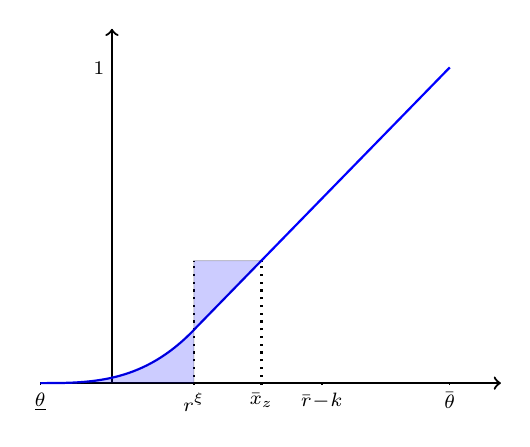
\begin{tikzpicture}[xscale=1.3, yscale=1]\scriptsize
\draw[->, thick] (0,0) -- (4.5,0);
\draw[->, thick] (0.7,0) -- (0.7,4.5) ;
% axis label
\draw [] (4,-.02)node[below]{$\bar\theta$}--(4,.02);
\draw [] (0,-.02)node[below]{$\underline\theta$}--(0,.02);
\draw [dotted, thick] (1.5,-.02)node[below]{$r^\xi$}--(1.5,1.556);

\draw [dotted, thick] (2.16,-.02)node[below]{$\bar x_z$}--(2.16,1.556);

\draw [thick] (2.75,-.02)node[below]{$\bar r-k$}--(2.75,.02);

\draw (0.7,4)node[anchor=east]{1};
% F
\draw[blue, domain=0:1.5,smooth,variable=\x, thick] plot ({\x},{.2*(\x)^3});

\draw[blue, domain=1.497:4,smooth,variable=\x, thick] plot ({\x},{1.3333*(\x)-1.324});

%Filling in regions
\draw[fill=blue,opacity=.2, domain=0:1.5,smooth,variable=\x] plot ({\x},{.2*(\x)^3})--(1.5,0)--(0,0);

\draw[fill=blue,opacity=.2, domain=1.497:2.16,smooth,variable=\x] plot ({\x},{1.3333*(\x)-1.324})--(1.5,1.556)--(1.5,.675);


\end{tikzpicture}	
\caption{$F_z^\xi$ for $z\in Z_B(k)$}
\label{fig:IC1}
\end{subfigure}
\hspace{20mm}
\begin{subfigure}[t]{0.4\textwidth}
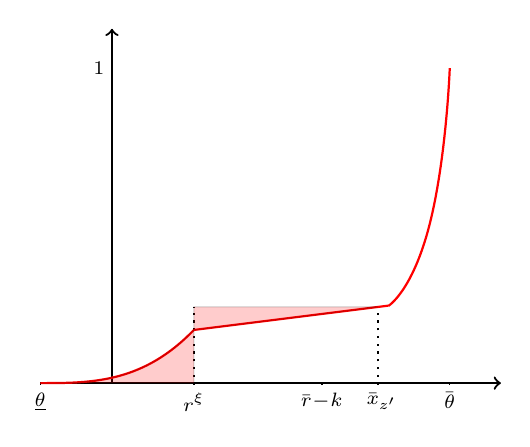
\begin{tikzpicture}[xscale=1.3, yscale=1]\scriptsize
\draw[->, thick] (0,0) -- (4.5,0);
\draw[->, thick] (0.7,0) -- (0.7,4.5) ;
% axis label
\draw [] (4,-.02)node[below]{$\bar\theta$}--(4,.02);
\draw [] (0,-.02)node[below]{$\underline\theta$}--(0,.02);
\draw [dotted, thick] (1.5,-.02)node[below]{$r^\xi$}--(1.5,.96755);

\draw [dotted, thick] (3.3,-.02)node[below]{~$\bar x_{z'}$}--(3.3,.96755);

\draw [thick] (2.75,-.02)node[below]{$\bar r-k$}--(2.75,.02);

\draw (0.7,4)node[anchor=east]{1};
% F
\draw[red, domain=0:1.5,smooth,variable=\x, thick] plot ({\x},{.2*(\x)^3});

\draw[red, domain=1.497:3.4,smooth,variable=\x, thick] plot ({\x},{.1625*(\x)+.4313});

\draw[red,thick,-] plot [smooth, tension=1] coordinates{(3.4,.98) (3.8, 2) (4, 4)};
% \draw[red, domain=3.5:4,smooth,variable=\x, thick] plot ({\x},{6*(\x)-20});

%Filling in regions
\draw[fill=red,opacity=.2, domain=0:1.5,smooth,variable=\x] plot ({\x},{.2*(\x)^3})--(1.5,0)--(0,0);

\draw[fill=red,opacity=.2, domain=1.497:3.3,smooth,variable=\x] plot ({\x},{.1625*(\x)+.4313})--(1.5,.96755)--(1.5,.675);

\end{tikzpicture}	
\caption{$F_{z'}^\xi$ for $z'\notin Z_B(k)$}
\label{fig:ICb}
\end{subfigure}
\captionsetup{singlelinecheck=false, justification=justified}
\caption{The two panels show the agent's interim posterior beliefs $F_z^\xi$ (in blue) and $F_{z'}^\xi$ (in red) after observing public signal realizations $z$ and $z'$, respectively. For ease of comparison, both $F_z^\xi$ and $F_{z'}^\xi$ have full support on $\Theta$ and $F_z^\xi(\theta)=F_{z'}^\xi(\theta)$ for all $\theta\leq r^\xi$. The point $\bar x_z$ is determined by the unique value such that the shaded area to the left of $r^\xi$  equals the shaded area to its right, i.e., $\int^{r^\xi}_{\underline \theta}F_z^\xi(\theta)d\theta=\int_{r^\xi}^{\bar x_z}[F_z^\xi(\bar x_z)-F_z(\theta)]d\theta$, and $\bar x_{z'}$ is defined~analogously.~As~$\bar x_z<\bar r-k<\bar x_{z'}$,~we~conclude that $z\in Z_B(k)$ and $z'\notin Z_B(k)$. }
\label{fig:ICbinds}
\end{center}
\end{figure}

 
 When $z\in Z_B(k)$, the principal must make a concession by offering a pass/fail signal $\pi(x_z)$ with  $x_z\in[r^\xi, \bar x_z]$ in order to persuade the agent. For any two cutoffs  $x_z'<x_z''$ in $[r^\xi, \bar x_z]$, the principal can charge more for $\pi(x_z')$ (as $x_z'$ is closer to the agent's actual reservation value of $r^\xi$) whereas she is more likely to keep the agent in the market by offering $\pi(x_z'')$ (as more goods are failed). Therefore, there is a familiar intra-temporal trade-off between surplus extraction (a higher per-period price) and persuasion (a higher probability of keeping the agent searching). Our proof of \autoref{prop:2} shows that the principal fully prioritizes persuasion when $z\in Z_B(k)$; she offers the pass/fail signal $\pi(\bar x_z)$, which makes the agent indifferent between stopping and continuing his search conditional on seeing a ``fail." As a result, the highest price the principal can charge to induce the agent to buy this signal is zero. The additional surplus loss in this case is captured by 
  \[
\int_{\bar x_z}^{\bar r-k}\big(\bar r-k-m\big)dF_Z^\xi(m)=\int_{\bar x_z}^{\bar r-k}\big(F^\xi_z(m)-F^\xi_z(\bar x_z)\big)dm,
 \]
 which in expectation yields the last term in \eqref{eq:5}.


In summary, a profit-maximizing principal wishes to induce a reservation value of $\bar r-k$ with the lowest possible $k\in [0, \bar r-r^\xi]$ for all realizations of the public signal. However, the principal can induce a reservation value of $\bar r-k$ only when the public signal realization $z\notin Z_A(k)\cup Z_B(k)$.  Therefore, the principal is able to induce the McCall reservation value in a stationary equilibrium following any public signal realization when $Z_A(0)\cup Z_B(0)$ is empty. In fact, we show a stronger result: the principal is able to induce the McCall reservation value if and only if $Z_A(k)\cup Z_B(k)$ is empty for all $k\in [0, \bar r-r^\xi]$. To see this, note that by construction, both $Z_A(k)$ and $Z_B(k)$ shrink (decrease in the inclusion order) as $k$ increases. Therefore, if $Z_A(k)\cup Z_B(k)$ is non-empty for some $k\in [0, \bar r-r^\xi]$, then $Z_A(k')\cup Z_B(k')$ is non-empty for all $k'\in[0,k]$. Thus, inefficiencies arise in a stationary equilibrium if and only if $Z_A(0)\cup Z_B(0)$ is non-empty,  and the efficiency loss is quantified by the unique solution to the fixed point $k=\delta\Phi(k)$.
 
 When $F_z^\xi$ has full support over $\Theta$ for all realizations $z\in Z,$ the set $Z_A(0)$ is trivially empty. The following result provides a sufficient and necessary condition for $Z_B(0)$ to also be empty in this case.


   
\begin{corollary}\label{cor:2}
        Consider a public signal $(\xi, Z)$ such that $F_z^\xi$ has full support on $\Theta$ for almost all $z\in Z$. The principal extracts the socially efficient surplus in a stationary equilibrium if and only if $\mathbb{E}_{F_z^\xi}[\theta|\theta\leq \bar r]\leq r^\xi$ for almost all $z\in Z$.
\end{corollary}

Intuitively, the requirement that $\mathbb{E}_{F_z^\xi}[\theta|\theta\leq \bar r]\leq r^\xi$ for almost all $z\in Z$ is equivalent to insisting that the interim posterior belief induced by almost each public signal realization has a relatively ``fat left tail," that is, the posterior belief places more mass below $r^\xi$ than it does on $[r^\xi, \bar r]$. This condition is trivially satisfied when the public signal is uninformative as $\mathbb{E}_F[\theta|\theta\leq \bar r]\leq \underline r\leq r(G)$ for any $G\in\mathcal{G}(F)$ and any absolutely continuous prior $F$. Hence, our result in \autoref{prop:1} can be seen as a special case of \autoref{prop:2}.

Of course, in some markets the agent may also observe a private signal about the quality of each object before deciding to contract with the principal. The agent's willingness-to-pay for an additional signal would then be his private information, introducing a screening problem \citep[as in][]{mus78} into each stage game between the principal and the agent. Such an analysis would require a different set of tools; for example, truth-telling constraints for a privately-informed agent would be more tractable if formulated via recommendation mechanisms \citep[as in][]{kol17} rather than via distributions of posterior means as in our analysis. We therefore view the study of private signals in search markets with endogenously-supplied information as a fruitful avenue for future research.



\section{Conclusion}\label{conclude}

In this paper, we introduce a persuaded search game in which a profit-maximizing principal with limited commitment controls the supply and pricing of information while an agent decides whether to acquire information from the principal and when to stop searching. By decentralizing information and decision-making in an otherwise workhorse model of sequential search without recall, our model highlights intra-temporal trade-offs between surplus extraction and persuasion as well as how these trade-offs are inter-temporally linked due to the dynamic considerations for both the principal and agent.

When the principal is the sole source of information, we show that the essentially unique stationary equilibrium  is efficient and features full surplus extraction by the principal. This also implies that the principal does not benefit from offering more complex contracts that condition prices on the signal realizations and agent's decision to stop or continue searching, considering non-stationary strategies, or having long-term commitment power.\footnote{ Despite the lack of private information in our setting, it is not a priori evident that the principal would be able to achieve as a high a payoff without commitment power; after all, the set of PBE outcomes could be a strict subset of the set of Nash equilibrium outcomes. Indeed, with long-term commitment power, the set of contracts that can be supported in equilibrium increases (in the set inclusion sense). For example, the principal could propose a sequence of contracts $\langle p_t, G_t\rangle_{t\geq 1}$ such that $G_t=F$ for all $t\geq 1$, $p_t=0$ for all $t>1$, and $p_1=\bar u-\underline u$. Such a sequence of contracts extracts the full surplus from the agent and is equivalent to ``selling the information production technology" to the agent. However, without long-term commitment power,  the principal would deviate away from charging $p_t=0$  in periods $t>1$, and thus, the agent would never accept the contract. }

In contrast, when there are public and free sources of additional information, we show that the essentially unique stationary equilibrium  could be inefficient, but only if the public information induces interim beliefs that are either too ``optimistic" or have a sufficiently ``thin left tail." Perhaps counterintuitively, this implies that while a free and public source of information never lowers the agent's ex-ante payoff, the agent may nevertheless end up with an ex-post lower-quality match. This finding matches the empirical results of \cite{hof18} who show that firms which use pre-employment tests along with additional sources of (public) information such as resume screening  end up hiring less productive employees than firms which rely only on pre-employment tests. While they attribute this result to human error or bias among hiring managers, our model predicts this as an equilibrium outcome of a contracting game between rational players.


The parsimonious and tractable nature of our model is useful to derive additional results under different settings. In the Online Appendix, we show that the qualitative properties of \autoref{prop:1} extend to a setting in which there is no discounting but the agent incurs a flow cost from searching. We also consider an alternative setting in which the principal and the agent have heterogeneous discount factors. We show that the essentially unique stationary equilibrium involves an inefficiently long search with ex-post higher-quality matches when the principal is more patient than the agent, whereas it involves an inefficiently short search with ex-post lower-quality matches when the principal is less patient than the agent. The tractability of our model also allows study of non-stationary equilibrium. In ongoing work, we characterize the set of all equilibrium payoffs. We show that for sufficiently low values of the discount factor $\delta$, all equilibria are payoff equivalent to the stationary equilibrium we characterize in \autoref{prop:1}, whereas for sufficiently high values of $\delta$, equilibrium payoffs emerge that can only be supported by non-stationary strategies.




 Of course, some search markets will contain different salient features that are not present in our model. For example, our model does not address how competition amongst multiple principals affects the supply and the pricing of information. The features of equilibrium contracts may therefore differ in such environments, and further study with an appropriately enriched model of a persuaded search game may yield novel economic insights. 


\singlespacing
 \bibliographystyle{abbrvnat}
\nocite{}\bibliography{bibref}
\onehalfspacing

\section*{Appendix}\label{appendix}

\noindent\begin{proof}[Proof of \autoref{lemma:1}]~

\noindent ($\Leftarrow$) Suppose the agent never searches, i.e., $\underline u=\bar u$. Then $\bar u=m_\varnothing$ because $\underline u=m_\varnothing$. Suppose for contradiction that $\underline \theta<\delta m_\varnothing$. Because $\bar u =m_\varnothing$ and because $\bar u$ is the solution to \eqref{eq:1} with $G=F$, we must have 
\begin{align*}
m_\varnothing=\int_\Theta \max\{m,\delta m_\varnothing\}dF(m)>\int_\Theta m dF(m) =m_\varnothing,
\end{align*}
where the strict inequality follows from $F$ having positive mass over the range $[\underline \theta, \delta m_\varnothing]$, and the second equality follows from the definition of $m_\varnothing$. This however yields the contradiction $m_\varnothing>m_\varnothing$. Hence, if the agent never searches then $\underline \theta\geq \delta m_\varnothing$.\\


\noindent ($\Rightarrow$)  Suppose $\underline\theta\geq \delta m_\varnothing$. Then for any $G\in\mathcal{G}(F)$, 
\begin{align*}
\int_\Theta\max\{m, \delta m_\varnothing\} dG(m)=\int_\Theta mdG(m)=m_\varnothing.
\end{align*}
Hence, $m_\varnothing$ is the solution to the fixed point problem in \eqref{eq:1}, i.e., $u(G)=m_\varnothing$ for all $G\in\mathcal{G}(F)$. In particular, $\bar u\triangleq u(F)=u(G^\varnothing)\triangleq\underline u$, so the agent never searches. 
\end{proof}\


% \begin{lemma}\label{lemma:binary}
% Let $G\in\mathcal{G}(F)$ be a solution to  \eqref{eq:4}. Then there exists a binary posterior-mean distribution $G^\dagger\in\mathcal{G}(F)$ with $\supp(G^\dagger)=\{m_1^\dagger, m_2^\dagger\}$ such that 
% \begin{enumerate}[$(i)$]
%     \item $m_1^\dagger\leq \underline r<m_2^\dagger$,
%     \item $G^\dagger$ is a mean-preserving contraction of $G$, and
%     \item $G^\dagger$ is a solution to \eqref{eq:4}.
% \end{enumerate}
% \end{lemma}

~

\noindent\begin{proof}[Proof of \autoref{lemma:binary}] Fix a distribution $G\in\mathcal{G}(F)$. 

\noindent ($\Rightarrow$) Suppose $G$ is a solution to \eqref{eq:4}. We construct a binary distribution satisfying points $(i)-(iv)$ of the lemma.

For any $V\geq 0$, we have 
\begin{align*}
    c_G(\underline r)-c_{G^\varnothing}(\underline r)+G(\underline r)\delta V \geq c_F(\underline r)-c_{G^\varnothing}(\underline r)+F(\underline r)\delta V>0
\end{align*}
where the first inequality is because $G$ solves \eqref{eq:4} and the last equality follows by \hyperref[ass:1]{Assumption 1}. We first argue that the agent must  both stop and continue his search in each period with a positive probability, i.e., $G(\underline r)\in (0,1)$. 

Suppose for contradiction that $G(\underline r)=0$, then 
\begin{align*}
    c_G(\underline r)&=c_G(\underline \theta)-\int_{\underline \theta}^{\underline r}\big(1-G(m)\big)dm \leq c_{G^\varnothing}(\underline \theta)-\int_{\underline \theta}^{\underline r}\big(1-G^{\varnothing}(m)\big)dm =c_{G^\varnothing}(\underline r),
\end{align*}
where the inequality follows because $c_G(\underline \theta)=c_{G^\varnothing}(\underline \theta)$ by point $(a)$ of  \autoref{remark:1} and because $0=G(m)\leq G^{\varnothing}(m)$ for all $m\leq \underline r$. Since $G^\varnothing$ is a mean-preserving contraction of $G$, we also have $c_G\geq c_{G^\varnothing}$ pointwise, which implies that $c_G(\underline r)=c_{G^\varnothing}(\underline r)$. However, this implies that $c_G(\underline r)-c_{G^\varnothing}(\underline r)+G(\underline r)\delta V=0$, which is a contradiction.

If instead $G(\underline r)=1$, then 
\[
c_G(\underline r)=\int^{\bar\theta}_{\underline r}\big(1-G(m)\big)dm=0
\]
while $c_{G^\varnothing}(\underline r)=m_\varnothing-\underline r=(1-\delta)m_\varnothing>0$. However, this contradicts the fact that $c_G\geq c_{G^\varnothing}$ pointwise. Therefore, we conclude that $G(\underline r)\in (0,1)$.

Consider the following binary distribution $G^\dagger$, which we will show satisfies points $(i)-(iv)$ of the lemma: 
\[
G^\dagger(m)=\left\{\begin{array}{ccl}
     0 &\mbox{if} &~~~ m<\mathbb{E}_{ G}[\theta|\theta\leq  \underline   r]  \\
        G(\underline r) &\mbox{if} &~~~ \mathbb{E}_{ G}[\theta|\theta\leq \underline r]\leq m<\mathbb{E}_{ G}[\theta|\theta> \underline r]  \\
     1 &\mbox{if} &~~~ m\geq \mathbb{E}_{ G}[\theta|\theta>  \underline r]
     \end{array}\right..
\]
The terms $\mathbb{E}_{ G}[\theta|\theta\leq  \underline   r]\triangleq m_1^\dagger$ and $\mathbb{E}_{ G}[\theta|\theta>  \underline r]\triangleq m_2^\dagger$ exist as $G(\underline r)\in (0,1)$, so $G^\dagger$ is well-defined. By construction, $m_1^\dagger<\underline r<m_2^\dagger$, establishing point $(i)$ of the lemma. Thus, $G^\dagger(\underline r)=G(\underline r)$, which by point $(d)$ of \autoref{remark:1} implies that $\partial_+c_{G^\dagger}(\underline r)=\partial_+c_G(\underline r)$, establishing point $(iii)$ of the lemma. 

It is straightforward to see that $G^\dagger$ is constructed as a mean-preserving contraction of $G$, and hence $c_{G^\varnothing}\leq c_{G^\dagger}\leq c_G$ pointwise. Additionally, notice that 
\begin{align*}
    c_G(\underline r)&=\int_{\underline r}^{\bar \theta}(m-\underline r)dG(m)\\[6pt]
    &=\big(\mathbb{E}_{G}[\theta|\theta\geq \underline r]-\underline r\big)\big(1-G(\underline r)\big)\\[6pt]
    &=\big(\mathbb{E}_{G}[\theta|\theta\geq \underline r]-\underline r\big)\big(1-G^\dagger(\underline r)\big)\\[6pt]
&=c_{G^\dagger}(\underline r).
\end{align*}
Therefore, we have established point $(ii)$ of the lemma.
We can now conclude that
\[
    c_G(\underline r)-c_{G^\varnothing}(\underline r)+G(\underline r)\delta V = c_{G^\dagger}(\underline r)-c_{G^\varnothing}(\underline r)+G^\dagger(\underline r)\delta V,
\]
so $G^\dagger$ is also a solution to \eqref{eq:4}, which establishes point $(iv)$ of the lemma, and completes the proof of existence of a binary distribution satisfying points $(i)-(iv)$. \\

\noindent ($\Leftarrow$) Suppose there exists a binary distribution $G^\dagger\in\mathcal{G}(F)$ satisfying points $(i)$-$(iv)$ of the lemma. Then $G$ solves \eqref{eq:4} because for all $\widehat G\in\mathcal{G}(F)$, 
\begin{align*}
    c_G(\underline r)-c_{G^\varnothing}(\underline r)+G(\underline r)\delta V &= c_{G^\dagger}(\underline r)-c_{G^\varnothing}(\underline r)+G^\dagger(\underline r)\delta V\geq c_{\widehat G}(\underline r)-c_{G^\varnothing}(\underline r)+\widehat G(\underline r)\delta V,
\end{align*}
where the equality holds by points $(ii)$ and $(iii)$ of the lemma while the inequality holds by point $(iv)$ of the lemma. %Thus, $G$ is also a solution to \eqref{eq:4}.
\end{proof}\\


\noindent\begin{proof}[Proof of \autoref{lemma:interval-x}]
For all $x\in \text{int}(\Theta)$, we have $\underline r=\delta\underline u<\underline u=\mathbb{E}_F[\theta] \leq \mathbb{E}_F[\theta|\theta>  x]$.  However, not all $x\in\text{int}(\Theta)$ satisfy $\mathbb{E}_F[\theta|\theta\leq x]\leq \underline r$. 
Since $F$ is assumed to be absolutely continuous, the function $x\mapsto \mathbb{E}_F[\theta|\theta\leq x]$ is continuous and strictly increasing. Additionally, $\mathbb{E}_F[\theta|\theta\leq \underline r]<\underline r<\mathbb{E}_F[\theta|\theta\leq \bar \theta]$. Hence, there is a unique point $\bar x\in(\underline r, \bar \theta)$ such that $\mathbb{E}_F[\theta|\theta\leq \bar x]=\underline r$, implying that  $\mathbb{E}_F[\theta|\theta\leq x]\leq \underline r<\mathbb{E}_F[\theta|\theta>  x]$ if and only if $x\leq \bar x$. 
 
We argued informally via \autoref{fig:44} that $c_G$ must be tangent to $c_F$ at some $x\in\text{int}(\Theta)$. We now show this claim formally: suppose for the sake of a contradiction that $G\in\mathcal{G}(F)$ solves \eqref{eq:4} and $c_G(x)<c_F(x)$ for all $x\in\text{int}(\Theta)$. From \autoref{lemma:binary}, $G$ has  support $\{m_1, m_2\}$ satisfying $\underline \theta<m_1\leq \underline r<m_2<\bar\theta$.\footnote{As $F$ is assumed to be absolutely continuous, no distribution $G\in \mathcal{G}(F)$ has positive mass at $\underline \theta$ or $\bar \theta$. Thus, $\underline\theta<m_1$ and $m_2<\bar \theta$.} Therefore, $G(\underline r)=G(m_1) \in (0,1).$ For $\epsilon >0$, consider a distribution $\widetilde G$ given by 
\[
\widetilde G(m)=\left\{\begin{array}{ccl}
     0 &\mbox{if} &~~~ m<m_1-(1-G(\underline r))\epsilon  \\
        G(\underline r) &\mbox{if} &~~~ m_1-(1-G(\underline r))\epsilon \leq m<m_2+G(\underline r)\epsilon  \\
     1 &\mbox{if} &~~~ m\geq m_2+G(\underline r)\epsilon 
     \end{array}\right..
\]
Notice $m_1-(1-G(\underline r))\epsilon<m_1\leq \underline r< m_2\leq m_2+G(\underline r)\epsilon$, so $\widetilde G(\underline r)=G(\underline r)$, which implies $\partial_+c_{\widetilde G}(\underline r)=\partial_+c_G(\underline r)$. Furthermore, by construction,  $c_G\leq c_{\widetilde G}$ pointwise, with $c_G(\underline r)<c_{\widetilde G}(\underline r)$. Finally, notice that $\lVert c_G-c_{\widetilde G}\rVert_\infty=G(\underline r)(1-G(\underline r))\epsilon<\epsilon$. Hence, for any $0<\epsilon\leq\lVert c_F-c_G\rVert$,  $c_{\widetilde G}\leq c_F$ pointwise, which implies that $\widetilde G\in\mathcal{G}(F)$. We have therefore found a feasible distribution that yields a strictly higher payoff in \eqref{eq:4} than $G$, which contradicts the assumption that $G$ is a solution to \eqref{eq:4}.

Therefore, any binary distribution $G$ that solves \eqref{eq:4} must have $c_G$ tangent to $c_F$ at some  $x\in\text{int}(\Theta)$, i.e., there exists some $x\in\text{int}(\Theta)$ such that $G=G^{\pi(x)}$. By point$(i)$ of \autoref{lemma:binary}, such a binary distribution $G^{\pi(x)}$ must have $ \mathbb{E}_F[\theta|\theta\leq x]\leq \underline r<\mathbb{E}_F[\theta|\theta>  x]$ so that  the agent is persuaded to continue searching when he observes a ``fail" and to stop when he observes a ``pass." Hence, $x\leq\bar x$. By the definition of $G^{\pi(\underline r)}$, we have that $c_{G^{\pi(\underline r)}}(\underline r)=c_F(\underline r)> c_{G^{\pi(x)}}(\underline r)$ for all $x\neq \underline r$. Additionally, for $x<\underline r$, we have $G^{\pi(x)}(\underline r)=F(x)<F(\underline r)=G^{\pi(\underline r)}(\underline r)$. In other words, for all $x<\underline r$, the value of \eqref{eq:4} evaluated at $G^{\pi(x)}$ is strictly lower than its value evaluated at $G^{\pi(\underline r)}$. Hence, $x\geq \underline r$.
\end{proof}\

~

\noindent\begin{proof}[Proof of \autoref{lemma:surplus_max}]
For any $x'\in\text{int}(\Theta)\backslash\{\bar r\}$,
\[
\bar r=\left(\frac{\delta}{1-\delta}\right)\cdot c_{F}(\bar r)=\left(\frac{\delta}{1-\delta}\right)\cdot c_{G^{\pi(\bar r)}}(\bar r)>\left(\frac{\delta}{1-\delta}\right)\cdot c_{G^{\pi(x')}}(\bar r)
\]
where the first equality follows because $\bar r$ is the unique solution to \eqref{eq:2} evaluated at $F$, the second equality follows because $c_{G^{\pi(\bar r)}}$ is tangent to $c_F$ at $\bar r$, and the strict inequality follows because $c_{G^{\pi(x')}}(x)=c_F(x)$ only for $x\in \{\underline \theta, x', \bar \theta\}$. Since $r(G^{\pi(\bar r)})$  is the unique solution to \eqref{eq:2} evaluated at $G^{\pi(\bar r)}$, we can conclude that $\bar r=r(G^{\pi(\bar r)})$. Similarly, $r(G^{\pi(x' )})$  is the unique solution to \eqref{eq:2} evaluated at $G^{\pi(x')}$, so $\bar r\neq r(G^{\pi(x')})$. In fact, since $\bar r$ is the highest possible reservation value, we conclude that $\bar r> r(G^{\pi(x')})$. Finally, because a reservation value is equal to the agent's discounted continuation value, we have $u(G^{\pi(x')})<u(G^{\pi(\bar r)})=\bar u$ for any $x'\in\text{int}(\Theta)\backslash\{\bar r\}$.
\end{proof}

~


\noindent \begin{proof}[Proof of \autoref{lemma:2}]
By  \hyperref[ass:1]{\Cref{ass:1}}, we have $\underline r<\bar r$. Hence, we need only prove $\bar r<\bar x$. By \autoref{lemma:interval-x}, proving that $\bar r< \bar x$  is equivalent to showing that
$\mathbb{E}_F[\theta|\theta\leq \bar r]<\underline r$. Suppose for contradiction that $\mathbb{E}_F[\theta|\theta\leq \bar r]\geq\underline r$. Then
\begin{align*}
\bar r&=\left(\frac{\delta}{1-\delta}\right)\cdot c_{G^{\pi(\bar r)}}(\bar r)\\[6pt]
&\leq \left(\frac{\delta}{1-\delta}\right)\cdot c_{G^{\pi(\bar r)}}(\mathbb{E}_F[\theta|\theta\leq \bar r])\\[6pt]
&=\left(\frac{\delta}{1-\delta}\right)\cdot c_{G^\varnothing}(\mathbb{E}_F[\theta|\theta\leq \bar r])\\[6pt]
&\leq \left(\frac{\delta}{1-\delta}\right)\cdot c_{G^\varnothing}(\underline r)\\[6pt]
&=\underline r,
\end{align*}
where the first equality follows because $\bar r=r(G^{\pi(\bar r)})$,  the first inequality follows because $c_{G^{\pi(\bar r)}}$ is weakly decreasing and $\mathbb{E}_F[\theta|\theta\leq \bar r]<\bar r$, the third equality follows because $c_{G^{\pi(\bar r)}}(x)=c_{G^\varnothing}(x)$ for all  $x\in \big[\underline \theta, \mathbb{E}_F[\theta|\theta\leq \bar r]\big]\cup \big[\mathbb{E}_F[\theta|\theta>\bar r], \bar \theta\big]$, the last inequality follows because $c_{G^\varnothing}$ is weakly decreasing and $\underline r\leq \mathbb{E}_F[\theta|\theta\leq \bar r]$ by assumption, and the last equality follows because $\underline r$ is the unique solution to \eqref{eq:2} evaluated at $G^\varnothing$. However, this yields $\bar r\leq \underline r$, which is not possible given \hyperref[ass:1]{\Cref{ass:1}}. Hence, $\mathbb{E}_F[\theta|\theta\leq \bar r]<\underline r$, which concludes the proof. 
\end{proof}\\

\noindent\begin{proof}[Proof of \autoref{prop:1}]
 \noindent It remains only to show sufficiency. To that end, suppose the principal proposes a contract $\langle p, G\rangle$ that satisfies points $(iii)$-$(v)$  of \autoref{prop:1} in every period following any history of events. Additionally, suppose the agent and the principal anticipate  continuation values satisfying $(i)$ and $(ii)$ of 
\autoref{prop:1}, i.e., $U=\underline u$ and $V=\bar u-\underline u$, respectively, following any history.
 We must show that \eqref{eq:os}, \eqref{eq:pc}, \eqref{eq:pm}, \eqref{eq:sga}, and \eqref{eq:sgp} are all satisfied.

As the agent anticipates the same continuation value $U=\underline u$ following any history of events, sequential rationality implies that he should stop searching in any given period if he samples a good whose expected quality satisfies $m>\delta \underline u=\underline r$. Hence, \eqref{eq:os} is satisfied. 

If the agent accepts the contract $\langle p, G\rangle$, he gets an expected utility of 
\begin{align*}
      \underline r+c_G( \underline r)-p &= \underline r+c_{G^{\pi(\bar r)}}(\underline r)-(\bar u-\underline u)\big(1-\delta F(\bar r)\big)\\[6pt]
     &= \underline r+c_{G^{\pi(\bar r)}}(\bar r)+\int^{\bar r}_{\underline r}\big(1-G^{\pi(\bar r)}(m)\big)dm-(\bar u-\underline u)\big(1-\delta F(\bar r)\big)\\[6pt]
     &= \underline r+c_{F}(\bar r)+(\bar r-\underline r)(1-F(\bar r))-(\bar u-\underline u)\big(1-\delta F(\bar r)\big)\\[6pt]
    &= \underline r+\left(\frac{1-\delta}{\delta}\right)\bar r+(\bar r-\underline r)(1-F(\bar r))-(\bar u-\underline u)\big(1-\delta F(\bar r)\big)\\[6pt]
    &=\underline r+\left(\frac{1-\delta}{\delta}\right)\underline r\\[6pt]
    &=\underline r+c_{G^\varnothing}(\underline r),
     \end{align*}
where the first equality follows by points $(iii)$ and $(v)$
 of the theorem, the second equality follows by breaking up the integral in $c_{G^{\pi(\bar r)}}(\underline r)$, the third equality follows because  $c_{G^{\pi(\bar r)}}$ is tangent to $c_F$ at $x=\bar r$ and because of \autoref{lemma:2}, the fourth equality follows because $\bar r$ is the unique reservation value that solves \eqref{eq:2} computed for $F$, and the last equality follows because $\underline r$ is the unique reservation value that solves \eqref{eq:2} computed for $G^\varnothing$. On the other hand, if the agent rejects the contract, he gets an expected utility of $\underline r+c_{G^\varnothing}(\underline r)$. Hence, the agent's participation constraint \eqref{eq:pc} binds for the contract $\langle p, G\rangle$. 
 
Given that the agent will accept the contract, his expected utility in any given period is 
\begin{align*}
\delta \underline u+c_G(\delta\underline u)-p=&\delta\underline u+c_{G^\varnothing}(\delta\underline u)\\
=&\underline u,
\end{align*}
where the first equality follows because the constraint \eqref{eq:pc} binds, and the second equality follows from \eqref{eq:1'}. Hence, the agent's self-generation condition \eqref{eq:sga} is satisfied.

Similarly, the principal's expected utility in any given period is
\begin{align*}
p+\delta G(\underline r)(\bar u-\underline u)=&(\bar u-\underline u)(1-\delta F(\bar r)) +\delta F(\bar r)(\bar u-\underline u)\\
=& \bar u-\underline u,
\end{align*}
where the first equality follows from $(iii)$ and $(iv)$ of \autoref{prop:1}. Hence, the principal's self-generation condition \eqref{eq:sgp} is also satisfied. Furthermore, since $\bar u-\underline u$ is the maximum payoff the principal can ever earn, \eqref{eq:pm} is also satisfied. Hence, a contract $\langle p, G\rangle$ satisfying $(iii)$-$(v)$ of \autoref{prop:1} along with a pair of continuation values $(U,V)=(\underline u, \bar u-\underline u)$ constitutes a stationary equilibrium. 
\end{proof}\\


\noindent\begin{proof}[Proof of \autoref{cor:1}]
From point $(iv)$ of \autoref{prop:1}, any  $G\in\mathcal{G}(F)$ that supports a stationary equilibrium must satisfy $G( \underline r)=F(\bar r)$, which implies by point $(d)$ of \autoref{remark:1} that $\partial_+ c_G( \underline r)=F(\bar r)-1$. Additionally, from point $(v)$ of \autoref{prop:1}, $c_G\geq c_{G^{\pi(\bar r)}}$  
pointwise. We also have $c_F\geq c_G$ pointwise for any $G\in\mathcal{G}(F)$. By construction, $c_F(\bar r)=c_{G^{\pi(\bar r)}}(\bar r)$, and $\partial_+ c_F( \bar r)=\partial_+ c_{G^{\pi(\bar r)}}( \bar r)=F(\bar r)-1$. Since $c_G$ is sandwiched between $c_F$ and $c_{G^{\bar r}}$, we have $\partial_+ c_G( \bar r)=F(\bar r)-1$ as well. 
Finally, by the convexity of $c_G$ (see point $(c)$ of \autoref{remark:1}), we have 
\[
\underbrace{\partial_+ c_G(\underline r)}_{=F(\bar r)-1}\hspace*{.5em}\leq \hspace*{.5em}\underbrace{\partial_+ c_G(x)}_{=G(x)-1}\hspace*{.5em}\leq \hspace*{.5em}\underbrace{\partial_+ c_G(\bar r)}_{=F(\bar r)-1}
\]for all $x\in [\underline r, \bar r]$. Equivalently, $G(x)=F(\bar r)$ for all $x\in [\underline r,  \bar r]$.
\end{proof}\\


\noindent\begin{proof}[Proof of \autoref{prop:2}]
     Suppose a family of contracts $\{\langle p_z,G_z\rangle\}_{z\in Z}$ 
 along with a pair of agent-principal continuation values $(U, V)$ constitute a stationary equilibrium. Since the objective function in \eqref{eq:pm2} is increasing in the price $\widehat p$, the constraint \eqref{eq:pc2} must   bind at the maximum, i.e., $p_z=c_{G_z}(\delta U)-c_{G_z^\varnothing}(\delta U)$ for all $z\in Z$. The fixed-point problem in \eqref{eq:sga2} then becomes  
\begin{align*}
U=&\delta U+\int_Z c_{G_z^\varnothing}(\delta U)\xi(dz)\\[6pt]
=&\delta U+c_{G^\xi}(\delta U),
\end{align*}
where the second equality holds because the mapping $G\to c_G$ is linear, which implies $\mathbb{E}_\xi[c_{G^\varnothing_z}(\cdot)]=c_{\mathbb{E}_\xi[G^\varnothing_z]}(\cdot)$, and by law of total probability, $\mathbb{E}_\xi[G^\varnothing_z]=G^\xi$. 
The above equality is the same as \eqref{eq:1'} evaluated at $G^\xi$ and thus has a unique solution $U=u(G^\xi)$, establishing point $(i)$ of the theorem. The agent's optimal stopping rule is then characterized by the reservation value $\delta u(G^\xi)\triangleq r^\xi$ from \eqref{eq:os}. 


In any equilibrium, the principal can always guarantee herself a payoff of zero and cannot extract more than the maximal surplus. Hence, the principal's stationary equilibrium continuation value satisfies $V\in [0, \bar u-u(G^\xi)]$. To prove point $(ii)$ of the theorem, we proceed in two steps: First, given the principal's  continuation payoff $V$, we characterize the principal's profit according to \eqref{eq:pm2} following any realization $z\in Z$ of the public signal. Second, we show that there is a unique $V$ that is consistent with the principal's self-generation condition \eqref{eq:sgp2}. \\

\noindent\textbf{Step 1:} Given the agent's reservation value and the binding constraint \eqref{eq:pc2}, the principal's profit maximization in \eqref{eq:pm2} following any $z\in Z$ can be expressed as 
\[
\label{eq:7}
\tag{7}
  G_z\in\argmax_{\widehat G\in \mathcal{G}(F^\xi_z)}\hspace*{.2em} c_{\widehat G}(r^\xi)-c_{G^\varnothing_z}(r^\xi)+ \widehat G(r^\xi) \delta V.
\]   
Let $\psi_z(V)$ represent the value function of \eqref{eq:7}. Below, we fully characterize the principal's value function for any public signal realization. To that end, we fix a public signal realization $z\in Z$ and consider three exhaustive cases depending on the support of the interim belief $F_z^\xi$:\\

\noindent \textbf{Case 1: $r^\xi<\underline \theta_z$.} In this case, the agent's interim belief is too optimistic as even the lowest quality possible given his beliefs will fall above his reservation value. Hence, he has no value for information and will stop his search with probability one. Formally, $c_{F^\xi_z}(x)=c_{G^\varnothing_z}(x)$ for all $x< \underline \theta_z$. Thus, for all $\widehat G\in\mathcal{G}(F^\xi_z)$, $c_{\widehat G}(r^\xi)=c_{G^\varnothing_z}(r^\xi)$ and $\widehat G(r^\xi)=G^\varnothing_z(r^\xi)=0$. Thus, $\psi_z(V)=0$ and the principal can achieve this value by offering contract $\langle p_z, G_z\rangle=\langle 0, G^\varnothing_z\rangle$. \\


\noindent \textbf{Case 2: $r^\xi>\bar \theta_z$.} In this case, the agent's interim belief is too pessimistic as even the highest quality possible given his beliefs will fall short of his reservation value. Hence, he has no value for information and will continue to search with probability one. 

Formally,  for all $\widehat G\in \mathcal{G}(F_z^\xi)$, $0=c_{F^\xi_z}(\underline \theta_z)\geq c_{F^\xi_z}(r^\xi)\geq c_{\widehat G}(r^\xi)\geq c_{G^\varnothing_z}(r^\xi)=0$, where the first inequality follows because $c_{F_z^\xi}$ is a weakly decreasing function, and the second and third inequalities follows because $c_{F_z^\xi}\geq c_{\widehat G}\geq c_{G^\varnothing_z}$ pointwise, and the last equality follows because $r^\xi>\underline\theta_z$. Hence, $c_{\widehat G}(r^\xi)=0$ which further implies $\widehat G(r^\xi)=1$. Thus, $\psi_z(V)=\delta V$ and the principal can achieve this value by offering contract $\langle p_z, G_z\rangle=\langle 0, G^\varnothing_z\rangle$.\\


\noindent \textbf{Case 3: $r^\xi\in [\underline \theta_z, \bar \theta_z]$.} 
In this case, the agent has a positive WTP for information, and thus is willing to contract with the principal. 
%In this case, the equilibrium distribution satisfies $G_z(r^\xi)\geq F_z^\xi(r^\xi)$. To see why, suppose for contradiction that $G_z(r^\xi)<F_z^\xi(r^\xi)$, then $\partial_+ c_{G_z}(r^\xi)<\partial_+c_{F_z^\xi}(r^\xi)$ (see Remark 1, point $(d)$) which, combined with $c_{G_z}\leq c_{F_z^\xi}$ pointwise, further implies that $c_{G_z}(r^\xi)<c_{F_z^\xi}(r^\xi)$. Then 
% \begin{align*}
%     \psi_z(V)&= c_{G_z}(r^\xi)-c_{G^\varnothing_z}(r^\xi)+ G_z(r^\xi) \delta V\\[6pt]
%     &<c_{F_z^\xi}(r^\xi)-c_{G^\varnothing_z}(r^\xi)+ F_z^\xi(r^\xi) \delta V.
% \end{align*}
% However, the strict inequality would contradict $G_z$ being the solution to \eqref{eq:7}. Hence, $G_z(r^\xi)\geq F_z^\xi(r^\xi)$. 
We next show that without loss of optimality, we can restrict attention to a sub-class of pass/fail signals $\{\pi(x_z)\}_{x_z\in [\underline \theta_z, \bar \theta_z]}$. 

\begin{lemma}\label{lemma_theorem_2_proof}
Suppose $r^\xi\in [\underline \theta_z, \bar \theta_z]$. Then the principal's value function can be attained by a pass/fail signal $\pi(x_z)$ for some $x_z\in [r^\xi, \bar x_z]$.
\end{lemma}
\begin{proof}[Proof of  \autoref{lemma_theorem_2_proof}]
The proof, which follows a similar argument to that of \autoref{lemma:interval-x}, is omitted.
\end{proof}

~

% \begin{lemma}\label{lemma_theorem_2_proof}
% Suppose $r^\xi\in [\underline \theta_z, \bar \theta_z]$. Then the principal's value function can be attained by a pass/fail signal such that for some $x_z\in [r^\xi, \bar\theta_z]$,  all goods of quality $\theta>x_z$ ``pass" while goods of quality $\theta\leq x_z$ ``fail."
% \end{lemma}
% \begin{proof}[Proof of  \autoref{lemma_theorem_2_proof}]
% As  $F_z^\xi$ does not have any atoms by assumption, there exists an  $x^*\in [r^\xi, \bar\theta_z]$ such that $G_z(r^\xi)=F_z^\xi(x^*)$. We proceed by showing that there exists a pass/fail signal with $x_z=x^*$ that attains the principal's value function $\psi_z(V).$

% If $x^*=\bar\theta_z$, then $G_z(r^\xi)=1$ and $c_{G_z}(r^\xi)=0$. Additionally, $c_{G_z}(r^\xi)\geq c_{G^\varnothing_z}(r^\xi)\geq 0$. Thus, $c_{G_z^\varnothing}(r^\xi)=0$, which implies $G^\varnothing_z(r^\xi)=1$ and $\mathbb{E}_{F_z^\xi}[\theta]=\mathbb{E}_{F_z^\xi}[\theta|\theta\leq x^*]\leq r^\xi$. We then have
% \begin{align*}
%     \psi_z(V)&= c_{G_z}(r^\xi)-c_{G^\varnothing_z}(r^\xi)+ G_z(r^\xi) \delta V=c_{G_z^\varnothing}(r^\xi)-c_{G^\varnothing_z}(r^\xi)+ G_z^\varnothing(r^\xi) \delta V.
% \end{align*}
% Thus, $G^\varnothing_z$ is also a solution to \eqref{eq:7}, which can be induced by a pass/fail signal that fails all goods, i.e., $x_z=x^*=\bar\theta_z$.


% If $x^*\in [r^\xi,\bar\theta_z)$, then $G_z(r^\xi)=F(x^*)<1$. By convexity of $c_{G_z}$, we have
% \begin{align*}
%     c_{G_z}(r^\xi)&\leq c_{G_z}(x^*)-\partial_+ c_{G_z}(r^\xi)(x^*-r^\xi)\\[6pt]
%     &=c_{G_z}(x^*)+\big(1-G_z(r^\xi)\big)(x^*-r^\xi)\\[6pt]
%         &\leq c_{F_z^\xi}(x^*)+\big(1-G_z(r^\xi)\big)(x^*-r^\xi)\\[6pt]
%     &= c_{F_z^\xi}(x^*)+\big(1-F_z^\xi(x)\big)(x^*-r^\xi)\\[6pt]
%     \label{eq:8}
%         \tag{8}
%     &=\big(1-F_z^\xi(x^*)\big)\big(\mathbb{E}_{F_z^\xi}[\theta|\theta>x^*]-r^\xi\big),
% \end{align*}
% where the first equality follows from point $(d)$ of \autoref{remark:1} and the second inequality follows because $c_{G_z}\leq c_{F_z^\xi}$ pointwise. Since $c_{G_z}(r^\xi)\geq c_{G^\varnothing_z}(r^\xi)=\max\{\mathbb{E}_{F_z^\xi}[\theta]-r^\xi, 0\}$ and $F_z^\xi(x^*)< 1$, we can conclude from \eqref{eq:8} that $\mathbb{E}_{F_z^\xi}[\theta|\theta\leq x^*]\leq r^\xi$.\footnote{Since $x^*\geq r^\xi$, it is trivially true that $\mathbb{E}_{F_z^\xi}[\theta|\theta>x^*]\geq r^\xi$.} 

% Consider a pass/fail signal with $x_z=x^*$, which induces the distribution $G_{x^*}$ given by 
% \[
% G_{x^*}(m)=\left\{\begin{array}{ccl}
%      0 &\mbox{if} & ~~~m<\mathbb{E}_{F_z^\xi}[\theta|\theta\leq  x^*]  \\
%        \underbrace{F_z^\xi(x^*)}_{=G_z(r^\xi)} &\mbox{if} &~~~ \mathbb{E}_{F_z^\xi}[\theta|\theta\leq  x^*]\leq m<\mathbb{E}_{F_z^\xi}[\theta|\theta>  x^*]  \\
%      1 &\mbox{if} & ~~~m\geq \mathbb{E}_{F_z^\xi}[\theta|\theta>  x^*]
%      \end{array}\right..
% \]
% It is then straightforward to show that 
% \begin{align*}
%     \psi_z(V)& = c_{G_z}(r^\xi)-c_{G^\varnothing_z}(r^\xi)+ G_z(r^\xi) \delta V\\[6pt]
%     &\leq c_{F_z^\xi}(x^*)+\big(1-F_z^\xi(x^*)\big)(x^*-r^\xi)-c_{G^\varnothing_z}(r^\xi)+ G_z(r^\xi) \delta V\\[6pt]
%     &= c_{F_z^\xi}(x^*)+\big(1-F_z^\xi(x^*)\big)(x^*-r^\xi)-c_{G^\varnothing_z}(r^\xi)+ F_z^\xi(x^*) \delta V\\[6pt]
%     &= c_{G_{x^*}}(r^\xi)-c_{G^\varnothing_z}(r^\xi)+ G_{x^*}(r^\xi) \delta V,
% \end{align*}
% where the inequality follows from \eqref{eq:8}. Hence, $G_{x^*}$ must also be a solution to \eqref{eq:7}, and it can be induced by a pass/fail signal with a cutoff $x_z=x^*$.
% \end{proof}

% Thus far, we have shown that following any realization $z\in Z$ such that $r^\xi\in [\underline \theta_z, \bar \theta_z]$, there exists a pass/fail signal such that the agent will continue his search if and only if the good ``fails." In other words, the posterior-mean distribution $G_{x_z}$ for some $x_z\in [r^\xi, \bar\theta_z]$ such that $\mathbb{E}_{F_z^\xi}[\theta|\theta\leq x_z]\leq r^\xi$ is a solution to \eqref{eq:7}. Recall $\bar x_z=\sup\{x\in [\underline \theta_z, \bar\theta_z]:\mathbb{E}_{F_z^\xi}[\theta|\theta\leq x]\leq r^\xi\}$. For any $x_z\leq \bar x_z$, the constraint on the conditional expectation is satisfied, i.e., $\mathbb{E}_{F_z^\xi}[\theta|\theta\leq x_z]\leq r^\xi$. 

We can now express the profit maximization problem in \eqref{eq:7} as solving for the optimal pass/fail cutoff:
\begin{align*}
% \label{eq:62}
% \tag{$6'$}
  x_z\in\argmax_{x\in [r^\xi, \bar x_z]}\hspace*{.2em} c_{F_z^\xi}(x)+\big(1-F_z^\xi(x)\big)(x-r^\xi)-c_{G^\varnothing_z}(r^\xi)+ F_z^\xi(x) \delta V.
\end{align*}  
 This objective function is (weakly) increasing for  $x<\delta V+r^\xi$ and (weakly) decreasing for $x>\delta V+r^\xi$. Thus, $x_z=\min\{\bar x_z, \delta V+r^\xi\}$ is a solution, and the principal's value function is 
\[
\psi_z(V)=\left\{\begin{array}{ccl}
 c_{F^\xi_z}(\delta V+r^\xi)-c_{G^\varnothing_z}(r^\xi)+\delta V &\mbox{if} & \delta V+r^\xi\leq \bar x_{z}\\
 F_z^\xi(\bar x_z)\delta V   & \mbox{if} &   \delta V+r^\xi> \bar x_{z}\end{array}\right..
\]
The first case (i.e., $\psi_z(V)=  c_{F^\xi_z}(\delta V+r^\xi)-c_{G^\varnothing_z}(r^\xi)+\delta V$ if $\delta V+r^\xi\leq \bar x_{z}$) follows directly from substituting $\delta V+r^\xi$ into the objective function for the optimal pass/fail cutoff. The second case (i.e., $\psi_z(V)= F_z^\xi(\bar x_z)\delta V$ if $\delta V+r^\xi> \bar x_{z}$) follows from the fact that
\begin{align*}
c_{F_z^\xi}(\bar x_z)+\big(1-F_z^\xi(\bar x_z)\big)(\bar x_z-r^\xi)&=\int^{\bar \theta_z}_{\bar x_z}(m-r^\xi)dF_z^\xi(m)\\[6pt]
&=\mathbb{E}_{F^\xi_z}[\theta]-r^\xi-\left(\mathbb{E}_{F^\xi_z}[\theta|\theta\leq \bar x_z]-r^\xi\right)F_z^\xi(\bar x_z)\\[6pt]
&=\max\{\mathbb{E}_{F_z^\xi}[\theta]-r^\xi, 0\}\\[6pt]
\label{eq:9}
\tag{8}
&= c_{G^\varnothing_z}(r^\xi)
\end{align*}
where the third equality follows because either $\mathbb{E}_{F_z^\xi}[\theta]\leq r^\xi$, in which case $\bar x_z=\bar\theta_z$ implying that $\mathbb{E}_{F^\xi_z}[\theta|\theta\leq \bar x_z]=\mathbb{E}_{F^\xi_z}[\theta]$ and $F_z^\xi(\bar x_z)=1$, or $\mathbb{E}_{F_z^\xi}[\theta]> r^\xi$, in which case $\bar x_z<\bar\theta_z$ and $\mathbb{E}_{F^\xi_z}[\theta|\theta\leq \bar x_z]=r^\xi$. This concludes Case 3.


We have now characterized the value function for all possible cases, which concludes Step 1. For convenience, we summarize below the principal's value function:
\small{\[
\psi_z(V)=\left\{\begin{array}{ccl}
  0&\mbox{if} & z\in Z_1\triangleq \{z'\in Z: r^\xi<\underline \theta_{z'}\}\\
\delta V&\mbox{if} &z\in Z_2\triangleq \{z' \in Z: r^\xi> \bar \theta_{z'}\}\\
    c_{F^\xi_z}(\delta V+r^\xi)-c_{G^\varnothing_z}(r^\xi)+\delta V &\mbox{if} &  z\in Z_3(V)\triangleq\{z'\in Z: r^\xi\in[\underline\theta_{z'}, \bar\theta_{z'}] \hspace*{.1em} \wedge \hspace*{.1em}  \bar x_{z'}\geq \delta V+r^\xi\} \\
  F_z^\xi(\bar x_z)\delta V   & \mbox{if} &  z\in Z_4(V)\triangleq\{z'\in Z: r^\xi\in[\underline\theta_{z'}, \bar\theta_{z'}] \hspace*{.1em} \wedge \hspace*{.1em}  \bar x_{z'}<\delta V+r^\xi\}
\end{array}\right..
\]}
\normalsize

\noindent \textbf{Step 2:} The principal's continuation value $V$ must be consistent with the principal's self-generation condition \eqref{eq:sgp2}, i.e., 
\small{\begin{align*}
 V=&\int_Z \psi_z(V)\xi(dz)\\[6pt]
    =& \delta V \xi(Z_2)+\int_{Z_3(V)}\left(c_{F^\xi_z}(\delta V+r^\xi)-c_{G^\varnothing_z}(r^\xi)+\delta V\right) \xi(dz) + \int_{Z_4(V)}\delta VF_z^\xi(\bar x_z) \xi(dz)\\[6pt]
    =&\int_{Z}\left(c_{F^\xi_z}(\delta V+r^\xi)-c_{G^\varnothing_z}(r^\xi)+\delta V \right)\xi(dz) -\int_{Z_1}\left(c_{F^\xi_z}(\delta V+r^\xi)-c_{G^\varnothing_z}(r^\xi)+\delta V \right)\xi(dz)\\[6pt]
    &-\int_{Z_2}\left(c_{F^\xi_z}(\delta V+r^\xi)-c_{G^\varnothing_z}(r^\xi)\right) \xi(dz)-\int_{Z_4(V)}\left(c_{F^\xi_z}(\delta V+r^\xi)-c_{G^\varnothing_z}(r^\xi)+\big(1-F_z^\xi(\bar x_z)\big)\delta V \right)\xi(dz)  \label{eq:10}
    \tag{9}.
\end{align*}}
\normalsize
Let us simplify each of these terms separately. The first term in \eqref{eq:10} simplifies to
\begin{align*}
    \int_{Z}\left(c_{F^\xi_z}(\delta V+r^\xi)-c_{G^\varnothing_z}(r^\xi)+\delta V\right) \xi(dz)&=c_{F}(\delta V+r^\xi)-c_{G^\xi}(r^\xi)+\delta V \\[6pt]
    &=c_{F}(\bar r)+\int_{\delta V+r^\xi}^{\bar r}\big(1-F(m)\big)dm-c_{G^\xi}(r^\xi)+\delta V\\[6pt]
    &=(1-\delta)\big(\bar u-u(G^\xi)\big)+\int_{\delta V+r^\xi}^{\bar r}\big(1-F(m)\big)dm +\delta V 
\end{align*}
where the first equality follows because the mapping $G\to c_G$ is linear and because $\mathbb{E}_\xi[F^\xi_z]=F$ and $\mathbb{E}_\xi[G^\varnothing_z]=G^\xi$, the second follows by breaking up the integral in the definition of $c_F(r^\xi+\delta V)$, and the last equality follows by evaluating \eqref{eq:1'} at $F$ and $G^\xi$.

For all $z\in Z_1$, we have $c_{F^\xi_z}(r^\xi)=c_{G^\varnothing_z}(r^\xi)$. Thus, the integrand of second term in \eqref{eq:10} simplifies to 
\begin{align*}
    c_{F^\xi_z}(\delta V+r^\xi)-c_{G^\varnothing_z}(r^\xi)+\delta V &=c_{F^\xi_z}(r^\xi)-\hspace*{-.5em}\int^{\delta V+r^\xi}_{r^\xi}\big(1-F_z^\xi(m)\big)dm-c_{G^\varnothing_z}(r^\xi)+\delta V\\[6pt]
    &=\int^{\delta V+r^\xi}_{r^\xi}\hspace*{-.5em}F_z^\xi(m)dm.
\end{align*}
Note that the above integral is non-zero only if $\delta V+r^\xi> \underline\theta_z$, which is equivalent to $z\in Z_A(\bar r-r^\xi-\delta V)$. 

For all $z\in Z_2$, we have $\delta V+r^\xi\geq r^\xi>\bar\theta_z$, which implies that $c_{F^\xi_z}(\delta V+r^\xi)=c_{G^\varnothing_z}(r^\xi)=0$. Thus, the third term in \eqref{eq:10} is zero.

Finally, for all $z\in Z_4(V)$, the integrand in the last term simplifies to 
\small{\begin{align*}
    c_{F^\xi_z}(\delta V+r^\xi)-c_{G^\varnothing_z}(r^\xi)+\big(1-F_z^\xi(\bar x_z)\big)\delta V &=c_{F^\xi_z}(\bar x_z)-\int^{\delta V+r^\xi}_{\bar x_z}\big(1-F_z^\xi(m)\big)dm-c_{G^\varnothing_z}(r^\xi)+\big(1-F_z^\xi(\bar x_z)\big)\delta V\\[6pt]
    &=\int^{\delta V+r^\xi}_{\bar x_z}\left(F_z^\xi(m)-F_z^\xi(\bar x_z)\right)dm,
\end{align*}}%
\normalsize
where the first equality follows by breaking up the integral in the definition of $c_{F^\xi_z}(\delta V+r^\xi)$ and the second equality follows from \eqref{eq:9}. Note that the above integral is non-zero only if $\bar\theta_z>\bar x_z$, which is equivalent to $z\in Z_B(\bar r-r^\xi-\delta V)$. 


Put together, we can write the expression in \eqref{eq:10} as 
\small{\begin{align*}
    V= &\bar u-u(G^\xi)+\frac{1}{1-\delta}\int_{\delta V+r^\xi}^{\bar r}1-F(m)dm\\[6pt]
    &-\frac{1}{1-\delta}\left(\int_{Z_A}\int^{\delta V+r^\xi}_{\underline\theta_z}F_z^\xi(m)dm \xi(dz)+\int_{Z_B}\int^{\delta V+r^\xi}_{\bar x_z}\left(F_z^\xi(m)-F_z^\xi(\bar x_z)\right)dm \xi(dz)\right)\\[6pt]
    =&\bar u-u(G^\xi)+\frac{k}{1-\delta}-\frac{1}{1-\delta}\Phi(k^*),
\end{align*}}%
\normalsize
where $\Phi(k)$ is as given in \eqref{eq:5}. The last equality follows by  using a change of variable $V=\bar u-u(G^\xi)-k^*/\delta$ so that $\delta V+r^\xi=\bar r-k^*$. Since we have both $V=\bar u-u(G^\xi)+k^*/(1-\delta)-\Phi(k^*)/(1-\delta)$ and $V=\bar u-u(G^\xi)-k^*/\delta$, it must be the case that $k^*$ solves the fixed point 
\[
k=\delta\Phi(k),
\]
which gives us the representation in \autoref{prop:2}. It remains to show such a solution exists and is unique. 
Note that if $\bar r=r^\xi$, then we just need to show that $\Phi(0)=0$, which is  trivially true as $Z_A(0)=Z_B(0)=\emptyset$. If $\bar r>r^\xi$, then $k-\delta\Phi(k)$ is continuous and strictly increasing in $k$ because both $Z_A(\cdot)$ and $Z_B(\cdot)$ are decreasing by construction (in the inclusion order). Additionally, 
\[
0-\delta\Phi(0)=-\delta\left(\int_{Z_A(k)}\int_{\underline \theta_z}^{\bar r}F^\xi_z(m)dm \hspace*{.2em}\xi(dz)+\int_{Z_B(0)}\int_{\bar x_z}^{\bar r}\left(F^\xi_z(m)-F^\xi_z(\bar x_z)\right)dm \hspace*{.2em}\xi(dz)\right)\leq 0.
\]
The first integral is non-negative because $\bar r>\underline\theta_z$ for all $z\in Z_A(0)$, and the second integral is non-negative because $\bar r>\bar x_z$ for all  $z\in Z_B(0)$. On the other hand, 
\[
\bar r-r^\xi-\delta\Phi(\bar r-r^\xi)=\int_{r^\xi}^{\bar r}
\big(1-\delta F(m)\big)dm>0
\] 
since $Z_A(\bar r-r^\xi)=Z_B(\bar r-r^\xi)=\emptyset$.
Thus, there exists a unique $k^*\in [0, \bar r-r^\xi]$ that solves the fixed point problem, which establishes point $(ii)$ of \autoref{prop:2} and completes Step 2.

We have found a unique pair $(U,V)$ and constructed a family of pass/fail signals that attains these values for the agent and principal, respectively, such that \autoref{def:2} is satisfied. Therefore, an equilibrium exists, completing the proof.
\end{proof}
  \endgroup


\end{document}